\section[Reguläre Sprachen und endliche Automaten]{Reguläre Sprachen und endliche Automaten\datenote{20.10.17}}
Wie können wir potentiell unendlich große Mengen von Wörtern darstellen?
Eine Lösung für dieses Problem sahen wir bereits im vorherigen Kapitel, als wir die (unendlich große) Menge der binär codierten Primzahlen mit Hilfe der folgenden Zeile darstellten.
\[
L_\mathsf{prim}=\{w\in\{0,1\}^*\mid w \text{ ist Binärcodierung einer Primzahl}\}
\]
Ein weiteres Beispiel ist die folgende Zeile.
\[
L_\mathsf{even}=\{w\in\{0,1\}^*\mid \text{ die Anzahl der Einsen in $w$ ist gerade. }\}
\]
Eine häufig interessante Fragestellung für ein gegebenes Wort $w$ und eine Sprache $L$ ist: "`Ist $w$ in $L$ enthalten?"' (Also: "`Gilt $w\in L$?"')
Wir nennen dieses Entscheidunsproblem das \emph{Wortproblem}. Eine konkrete Instanz des Wortproblems wäre z.B.\ "`$1100101\in L_\mathsf{prim}$?"' oder "`$1100101\in L_\mathsf{even}$?"'

Die obige Darstellung der unendlichen Mengen $L_\mathsf{prim}$ und $L_\mathsf{even}$ ist zwar sehr kompakt, 
wir können daraus aber nicht direkt ein Vorgehen zur Lösung des Wortproblems ableiten.
Wir müssen zunächst verstehen, was die Begriffe "`Binärcodierung"', "`Primzahl"' oder "`gerade Anzahl"' bedeuten und für $L_\mathsf{prim}$ und $L_\mathsf{even}$ jeweils einen Algorithmus zur Entscheidung entwickeln.

In diesem Kapitel werden wir mit \emph{endlichen Automaten} einen weiteren Formalismus kennenlernen, um (potentiell unendlich große) Mengen von Wörtern darzustellen. 
Ein Vorteil dieser Darstellung ist, dass es einen einheitlichen und effizienten Algorithmus für das Wortproblem gibt.
Wir werden aber auch sehen, dass sich nicht jede Sprache (z.B.\ $L_\mathsf{prim}$) mit Hilfe eines endlichen Automaten darstellen lässt.

\subsection{Endliche Automaten}
Wir beschreiben zunächst informell die Bestandteile eines endlichen Automaten:

\newcommand{\qinit}{{q^\mathsf{init}}}
\newcommand{\B}{\mathcal{B}}
\newcommand{\calN}{\mathcal{N}}
\newcommand{\calP}{\mathcal{P}}
\newcommand{\ecl}{\textsf{ecl}}
\newcommand{\reach}{\textsf{reach}}
\newcommand{\hide}[1]{}

\begin{description}
\item[Endliches Band] 
(read-only; jede Zelle enthält ein $a_i\in\Sigma$; der Inhalt des Bands ist das \emph{Eingabewort} bzw.\ die \emph{Eingabe})

\begin{figure}[H]\centering
        \begin{tikzpicture}
                \node (A) [block]{$a_0$};
                \node (B) [block,right=of A] {$\dots$};
                \node (C) [block,right=of B] {$a_n$};

    \node (L) [above=of A, node distance = 0.25cm] {Lesekopf};
    \draw[->] (L) -- (A);
        \end{tikzpicture}
        \caption{Endliches Band}
\end{figure}
\vspace{-1em}
\item[Lesekopf] ~\\
  \vspace{-\baselineskip}
  \begin{itemize}
        \item Der \emph{Lesekopf} zeigt auf ein Feld des Bands, oder hinter das letzte Feld.
        \item Er bewegt sich feldweise nach rechts; andere Bewegungen (Vor- bzw.\ Zurückspulen) sind nicht möglich.
        \item Wenn er hinter das letzte Zeichen zeigt, \emph{stoppt} der Automat.
    Er muss sich nun "`entscheiden"' ob er das Wort \emph{akzeptiert} oder nicht.
  \end{itemize}
\item[Zustände] $q$ aus \emph{endlicher} Zustandsmenge $Q$
\item[Startzustand] $\qinit \in Q$
\item[Akzeptierende Zustände] $F \subseteq Q$ 
\item[Transitionsfunktion] Im Zustand $q$ beim Lesen von $a$ gehe in Zustand $\delta(q) = q'$.
\end{description}
Der endliche Automat akzeptiert eine Eingabe, falls er in einem akzeptierenden Zustand stoppt.

% Spiral - By Keven Law - originally posted to Flickr as What's your Colour???, CC BY-SA 2.0, https://commons.wikimedia.org/w/index.php?curid=6851868
% Bunch - By Mariajudit - Own work, CC BY-SA 4.0, https://commons.wikimedia.org/w/index.php?curid=48726001
% Almond - By Michelle Naherny - Own work, CC BY-SA 4.0, https://commons.wikimedia.org/w/index.php?curid=44361114
\needspace{5\baselineskip}
\begin{Bsp}Aufgabe: 
  \\
  \label{Bsp:3.1}
  "`Erkenne alle Stapel von Macarons, in denen höchstens ein grünes Macaron vorkommt."'
\begin{center}
  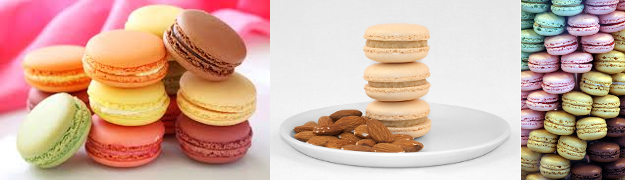
\includegraphics[scale=0.4]{macaron-stacks.png}~\footnote{
  \tiny Von links nach rechts: \\
By Mariajudit - Own work, CC BY-SA 4.0, https://commons.wikimedia.org/w/index.php?curid=48726001
  \\
By Michelle Naherny - Own work, CC BY-SA 4.0, https://commons.wikimedia.org/w/index.php?curid=44361114
  \\
By Keven Law - originally posted to Flickr as What's your Colour???, CC BY-SA 2.0, \\ https://commons.wikimedia.org/w/index.php?curid=6851868
}
% Bunch - By Mariajudit - Own work, CC BY-SA 4.0, https://commons.wikimedia.org/w/index.php?curid=48726001
% Almond - By Michelle Naherny - Own work, CC BY-SA 4.0, https://commons.wikimedia.org/w/index.php?curid=44361114

\end{center}
Ein passendes Alphabet wäre $\Sigma = \{\texttt{grün} , \texttt{nicht-grün} \}$.
Wir definieren die folgenden Zustände.
(Die Metapher hier ist: "`wenn ich mehr als ein grünes Macaron esse, wird mir übel, und das wäre nicht akzeptabel"'.)
\begin{center}
\begin{tabular}{cl}
  Zustand & Bedeutung \\
  \hline
  $q_0$& "`alles gut"' \\
  $q_1$& "`mir wird schon flau"' \\
  $q_2$& "`mir ist übel"'
\end{tabular}
\end{center}
Der Startzustand ist $q_0$.
Akzeptierende Zustände sind $q_0$ und $q_1$.
Die Transitionsfunktion $\delta$ ist durch die folgende Tabelle gegeben.
\begin{center}
\begin{tabular}{cccl}
  &\texttt{grün} & \texttt{nicht-grün} \\
  \hline
  $q_0$ & $q_1$ & $q_0$ & wechsle nach $q_1$ falls \texttt{grün}, ansonsten verweile \\
  $q_1$ & $q_2$ & $q_1$ & wechsle nach $q_2$ falls \texttt{grün}, ansonsten verweile \\
  $q_2$  & $q_2$ & $q_2$ & verweile, da es nichts mehr zu retten gibt
\qedhere
\end{tabular}
\end{center}
\end{Bsp}

% \begin{Bsp}
%       $L=\{w\in\{0,1\}^* \mid w \text{ enthält gerade Anzahl von 0 und gerade Anzahl von 1}\}$

%       \begin{minipage}[t]{.4\textwidth}\centering\vspace{0pt}
%           \captionsetup{type=figure}
%               \begin{tikzpicture}[circle/.style={
%                       shape=circle,
%                       minimum size=0.5cm,
%                       text=black, draw,
%                       text width=0.5cm,
%                       align=center}]
%                       \node (v1) at (-3.5,3.5) {};
%                       \node [circle,double] (v2) at (-2.5,3) {$q_{00}$};
%                       \node [circle] (v3) at (0.5,3) {$q_{01}$};
%                       \node [circle] (v4) at (0.5,0.5) {$q_{10}$};
%                       \node [circle] (v5) at (-2.5,0.5) {$q_{11}$};
%                       \draw [->] (v1) edge (v2);
%                       \draw [->] (v2) edge [bend left=15] node[auto] {1} (v3);
%                       \draw [->] (v3) edge [bend left=15] node[auto] {1} (v2);
%                       \draw [->] (v3) edge [bend left=15] node[auto] {0} (v4);
%                       \draw [->] (v4) edge [bend left=15] node[auto] {0} (v3);
%                       \draw [->] (v2) edge [bend left=15] node[auto] {0} (v5);
%                       \draw [->] (v5) edge [bend left=15] node[auto] {0} (v2);
%                       \draw [->] (v5) edge [bend left=15] node[auto] {1} (v4);
%                       \draw [->] (v4) edge [bend left=15] node[auto] {1} (v5);
%               \end{tikzpicture}
%               \captionof{figure}{Automat zu $L$}
%       \end{minipage}\begin{minipage}[t]{.55\textwidth}\vspace{0pt}
%       Graphische Darstellung $\hat=$ gerichteter Graph mit Knoten $Q$ und markierten Kanten gemäß $\delta$.\\
%       $Q=\{q_{00},q_{01},q_{10},q_{11}\}$\\
%       $q_{00}$ einziger akzeptierender Zustand ($F=\{q_{00}\}$)
%       \end{minipage}
        
%       \begin{tabular}{M{l}|M{l}|M{l}l @{\quad}l}
%               & 0 & 1 &\\ \cline{1-3}
%               q_{00} & q_{10} & q_{01} && gerade Anzahl von 0 und 1 gesehen\\
%               q_{01} & q_{11} & q_{00} && gerade \ruleplaceholder{\widthof{Anzahl von 0}}, ungerade Anzahl von 1 gesehen\\
%               q_{10} & q_{00} & q_{11} && ungerade \ruleplaceholder{\widthof{Anzahl von 0}}, gerade \ruleplaceholder{\widthof{Anzahl von 1 gesehen}} \\
%               q_{11} & q_{01} & q_{10} && ungerade \ruleplaceholder{\widthof{Anzahl von 0}}, ungerade \ruleplaceholder{\widthof{Anzahl von 1 gesehen}}
%       \end{tabular}
% \end{Bsp}
\begin{Def}[\acs*{DEA}]
        Ein \emph{\acf{DEA}}, (\acsu{DFA} $\hat=$ \acl{DFA}) ist ein 5-Tupel
        \[ \A= (\Sigma, Q,\delta,\qinit,F). \]
Dabei ist
        \begin{itemize}
                \item $\Sigma$ ein Alphabet,
                \item $Q$ eine \emph{endliche} Menge, deren Elemente wir \emph{Zustände} nennen,
                \item $\delta:Q\x\Sigma\->Q$ eine Funktion, die wir \emph{Transitionsfunktion} nennen,
                \item $\qinit\in Q$ ein Zustand, den wir \emph{Startzustand} nennen und
                \item $F\subseteq Q$ eine Teilmenge der Zustände, deren Elemente wir \emph{akzeptierende} Zustände nennen.
                \qedhere
        \end{itemize}
\end{Def}

\acs*{DEA}s lassen sich auch graphisch darstellen.
Dabei gibt man für den Automaten einen gerichteten Graphen an.
Die Knoten des Graphen sind die Zustände, und mit Zeichen beschriftete Kanten zeigen, welchen Zustandsübergang die Transitionsfunktion für das nächste Zeichen erlaubt.
Der Startzustand ist mit einem unbeschrifteten Pfeil markiert, akzeptierende Zustände sind doppelt eingekreist.
Hier ist die graphische Darstellung von $A_{\mathtt{Macaron}}$ aus Beispiel~\ref{Bsp:3.1}:

\begin{center}
\begin{tikzpicture}[node distance = 3cm]
  \node[state, accepting] (0) {$q_0$};
  \node[state, accepting, right of = 0] (1) {$q_1$};
  \node[state, right of = 1] (2) {$q_2$};

  \node[left of = 0, node distance = 1cm] (start){}; 
  \draw[->] (start) to (0);

  \draw[->] (0) to node[above] {\texttt{grün}} (1);
  \draw[->, loop above] (0) to node[above] {\texttt{nicht-grün}} (0);

  \draw[->] (1) to node[above] {\texttt{grün}} (2);
  \draw[->, loop above] (1) to node[above] {\texttt{nicht-grün}} (1);

  \draw[->, loop right] (2) to node[right]{\texttt{grün}, \texttt{nicht-grün}} (2);
\end{tikzpicture}
\end{center}

% \acs*{DEA}s charakterisieren die Sprachen durch die Menge an Wörtern, die sie akzeptieren.
Die folgenden beiden Definitionen erlauben uns mit Hilfe eines \acs*{DEA} eine Sprache zu charakterisieren.
% \begin{Bsp}
%     Sei $M=(\Sigma, Q,\delta,q_0,F)$ ein \acs*{DEA}.
%     \begin{itemize}
%     \item Wenn $F=Q$, dann ist $L(M)=\Sigma^*$.
%     \item Wenn $F=\emptyset$, dann ist $L(M)=\emptyset$.
%     \end{itemize}
% \end{Bsp}
\begin{Def}[name={[Induktive erweiterung von $\delta$ auf Wörter]}]\label{def:2.deltaschlange}
        Die \emph{induktive Erweiterung} von $\delta:Q\x\Sigma\->Q$ auf Wörter, $\tilde{\delta}: Q\x\Sigma^*\->Q$, ist (induktiv) definiert durch
  \begin{enumerate}
  \item $\tilde\delta(q,\Eps) =q$\ \ \ \  (Wortende erreicht)
  \item $\tilde\delta(q,aw)=\tilde\delta(\delta(q,a),w)$\ \ \ \ (Rest im Folgezustand verarbeiten)
  \qedhere
  \end{enumerate}
\end{Def}
\begin{Def}[name={[Die durch einen \acs*{DEA} akzeptierte Sprache]}]\label{def:2.sprache}
        Sei $\A=(\Sigma, Q,\delta,\qinit,F)$. 
        Ein Wort $w\in\Sigma^*$ wird von $\A$ \emph{akzeptiert}, falls $\tilde\delta(\qinit,w)\in F$.
        Die \emph{von $\A$ akzeptierte Sprache}, geschrieben $L(\A)$, ist die Menge aller Wörter, die von $\A$ akzeptiert werden. D.h., 
        \[ L(\A) = \{ w\in\Sigma^* \mid \tilde\delta(\qinit,w)\in F \}. \]
        Eine durch einen \acs*{DEA} akzeptierte Sprache heißt \emph{regulär}.
\end{Def}

\begin{Bsp} 
\label{bsp:3.1} Ein möglicher \acs*{DEA} für die Sprache 
$$L_\mathsf{even}=\{w\in\{0,1\}^*\mid \text{ die Anzahl der Einsen in $w$ ist gerade. }\}$$ 
aus der Einleitung dieses Kapitels hat die folgende graphische Repräsentation.
%         $L=\{w\in\{0,1\}^* \mid w \text{ enthält gerade Anzahl von 0 und gerade Anzahl von 1}\}$
  \begin{center}
                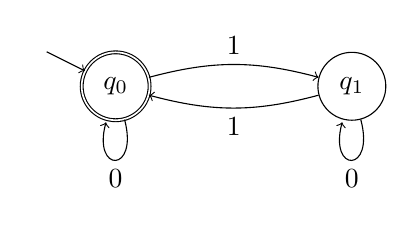
\begin{tikzpicture}[circle/.style={
                        shape=circle,
                        minimum size=0.5cm,
                        text=black, draw,
                        text width=0.5cm,
                        align=center}]
                        \node (v1) at (-3.5,3.5) {};
                        \node [circle,double] (v2) at (-2.5,3) {$q_{0}$};
                        \node [circle] (v3) at (0.5,3) {$q_{1}$};
                        \draw [->] (v1) edge (v2);
                        \draw [->] (v2) edge [bend left=15] node[auto] {1} (v3);
                        \draw [->] (v3) edge [bend left=15] node[auto] {1} (v2);
%                         \draw [->] (v1) edge [bend left=15] node[auto] {0} (v1);
%                         \draw [->] (v2) edge [bend left=15] node[auto] {0} (v1);
                        \draw [->] (v2) edge [loop below] node[auto] {0} (v2);
                        \draw [->] (v3) edge [loop below] node[auto] {0} (v3);
                \qedhere
                \end{tikzpicture}
  \end{center}
\end{Bsp}



% Es folgen zwei Beispiele für reguläre Sprachen:
% \begin{Bsp} 
% \label{bsp:3.1}
%         $L=\{w\in\{0,1\}^* \mid w \text{ enthält gerade Anzahl von 0 und gerade Anzahl von 1}\}$
%   \begin{center}
%                 \begin{tikzpicture}[circle/.style={
%                         shape=circle,
%                         minimum size=0.5cm,
%                         text=black, draw,
%                         text width=0.5cm,
%                         align=center}]
%                         \node (v1) at (-3.5,3.5) {};
%                         \node [circle,double] (v2) at (-2.5,3) {$q_{00}$};
%                         \node [circle] (v3) at (0.5,3) {$q_{01}$};
%                         \node [circle] (v4) at (0.5,0.5) {$q_{10}$};
%                         \node [circle] (v5) at (-2.5,0.5) {$q_{11}$};
%                         \draw [->] (v1) edge (v2);
%                         \draw [->] (v2) edge [bend left=15] node[auto] {1} (v3);
%                         \draw [->] (v3) edge [bend left=15] node[auto] {1} (v2);
%                         \draw [->] (v3) edge [bend left=15] node[auto] {0} (v4);
%                         \draw [->] (v4) edge [bend left=15] node[auto] {0} (v3);
%                         \draw [->] (v2) edge [bend left=15] node[auto] {0} (v5);
%                         \draw [->] (v5) edge [bend left=15] node[auto] {0} (v2);
%                         \draw [->] (v5) edge [bend left=15] node[auto] {1} (v4);
%                         \draw [->] (v4) edge [bend left=15] node[auto] {1} (v5);
%                 \end{tikzpicture}
%   \end{center}
% \end{Bsp}
% \begin{Bsp}\label{bsp:3.2}
%         
%         Sei $A\ge 0$ nat. Zahl, $\Sigma=\{0,1,\dots,A\}$
%         \begin{equation*}
%                 L = \{ a_1\dots a_n \mid \exists J\subseteq \{1,\dots,n \}: \sum_{i\in J} a_i = A \} \subseteq \Sigma^* 
%         \end{equation*}
%         D.h.\ gegeben eine Liste von Zahlen $\in\Sigma$.
%         Akzeptiere diejenigen Listen, für die eine Teilliste existiert, deren Summe genau $A$ ist.
%         \begin{align*}
%                 Q &=\Powerset\{0,1,\dots,A\} \\
%                 \delta(q,a) &= q \cup \{ x\in \{0,\dots,A\} \mid x-a \in q \} \\
%                 q_0 &=\{0\} \\
%                 F &= \{ q\in Q \mid A \in q \}
%         \end{align*}
%   $q \in Q$ bezeichnet die Menge an möglichen Summen $\le A$, die mit den bisher gelesenen Zeichen gebildet werden kann.
%   Die Transitionsfunktion $\delta$ fügt die Summen zum aktuellen Zustand hinzu, die sich durch addieren der aktuell gelesenen Ziffer zu den alten Möglichkeiten ergeben.
% \end{Bsp}
% \begin{Bsp}\label{bsp:3.3}
%         Beispiel für eine nicht-reguläre Sprache.
%         \begin{equation*}
%                 L = \{ 0^n1^n \mid n\in\N \} 
%         \end{equation*}
%         erkennbar durch \ac{TM} die immer anhält, \emph{aber nicht} von einem \ac{DEA} [\emph{nicht} regulär] akzeptiert werden kann.
%         \begin{proof}
%                 Angenommen $L=L(M)$ für \ac{DEA} $M=(\Sigma, Q,q_0,\delta,F)$
%                 
%                 Beobachtung: $\exists m\neq n$, sodass $\tilde\delta(q_0,0^m)=\tilde\delta(q_0,0^n)=q'$ weil $Q$ endlich.
%                 \begin{itemize}
%                         \item Falls nun $\tilde\delta(q',1^m)\in F$, dann ist auch $\tilde\delta(q_0,0^n1^m)\in F$ und somit $0^n1^m\in L(M)$ mit $n\neq m\ \lightning$
%                         \item Falls $\tilde\delta(q',1^m)\notin F$, dann gilt auch $\tilde\delta(q_0,0^m1^m)\notin F$ und somit $0^m1^m \notin L$ $\lightning$
%                 \end{itemize}
%                 Also kann $M$ nicht existieren!
%         \end{proof}
% \end{Bsp}


Frage: Gegeben seien zwei reguläre Sprachen $L_1$, $L_2$ über einem gemeinsamen Alphabet $\Sigma$; ist dann auch der Schnitt $L_1\cap L_2$ eine reguläre Sprache? Wir beantworten diese Frage mit dem folgenden Satz.

\begin{Satz}\label{satz:2.ClosedIntersection}
  Reguläre Sprachen sind abgeschlossen unter der Schnittoperation. (D.h.\ für zwei gegebene reguläre Sprachen $L_1$, $L_2$ über $\Sigma$ ist auch der Schnitt $L_1\cap L_2$ eine reguläre Sprache.)
\end{Satz}

% Der folgende Beweis ist ein typi

\begin{proof}\footnote{Dieser erste Beweis ist außergewöhnlich detailliert. Im den folgenden Beweisen werden wir einfache Umformungen zusammenfassen.}
Da $L_1$ und $L_2$ regulär sind, gibt es zwei \ac{DEA}s $A_1=(\Sigma, Q_1,\delta_1,\qinit_1,F_1)$ und $A_2=(\Sigma, Q_2,\delta_2,\qinit_2,F_2)$ mit $L_1=L(A_1)$ und $L_2=L(A_2)$.
Wir konstruieren nun zunächst den \emph{Produktautomaten für Schnitt} $A_\cap=(\Sigma, Q_\cap,\delta_\cap,\qinit_\cap,F_\cap)$ wie folgt.
		\begin{align*}
			Q_\cap &= Q_1\x Q_2\\
			\delta_\cap((q_1,q_2),a) &= (\delta_1(q_1,a),\delta_2(q_2,a))\;, \quad \text{für alle } a\in\Sigma\\
			\qinit_\cap &= (\qinit_1,\qinit_2)\\
			F_\cap &= F_1\x F_2\\
		\end{align*}
Anschließend zeigen wir, dass $L(A_\cap)=L(A_1)\cap L(A_2)$ gilt. 
Hierfür zeigen wir zunächst via Induktion über die Länge von $w$, dass für alle $w\in\Sigma^*$, für alle $q_1\in Q_1$ und für alle $q_2\in Q_2$ die folgende Gleichung gilt.
$$\tilde{\delta}_\cap((q_1,q_2),w) = (\tilde{\delta}_1(q_1,w), \tilde{\delta}_2(q_2,w))$$
Der Induktionsanfang für $n=0$ folgt dabei direkt aus \autoref{def:2.deltaschlange}, da $\Eps$ das einzige Wort der Länge $0$ ist.
$$\tilde{\delta}_\cap((q_1,q_2),\Eps) = (q_1,q_2)$$
Den Induktionsschritt $n\rightsquigarrow n+1$ zeigen wir mit Hilfe der folgenden Umformungen, wobei $a\in\Sigma$ ein beliebiges Zeichen und $w\in\Sigma^n$ ein beliebiges Wort der Länge $n$ ist.
\begin{eqnarray*}
  \tilde{\delta}_\cap((q_1,q_2),aw) 
    & \stackrel{\text{\autoref{def:2.deltaschlange}}}{=} & \tilde{\delta}_\cap(\delta_\cap((q_1,q_2),a),w)\\
    & \stackrel{\text{Def.\ }\delta_\cap}{=} & \tilde{\delta}_\cap (\big(\delta_1(q_1,a),\delta_2(q_2,a)\big),w)\\
    & \stackrel{\text{I.V.}}{=} & \big(\tilde{\delta}_1 (\delta_1(q_1,a),w), \tilde{\delta}_2(\delta_2(q_2,a),w)\big)\\
    & \stackrel{\text{\autoref{def:2.deltaschlange}}}{=} & \big(\tilde{\delta}_1(q_1,aw), \tilde{\delta}_2(q_2,aw)\big)
\end{eqnarray*}
Schließlich zeigen wir $L(A_\cap)=L(A_1)\cap L(A_2)$ mit Hilfe der folgenden Umformungen für ein beliebiges $w\in\Sigma^*$.
\begin{eqnarray*}
  w\in L(A_\cap)
  & \stackrel{\text{\autoref{def:2.sprache}}}{\mathsf{gdw}} & \tilde{\delta}_\cap(\qinit_\cap,w)\in F_\cap\\
  & \stackrel{\text{Def.\ }\qinit_\cap}{\mathsf{gdw}} & \tilde{\delta}_\cap((\qinit_1,\qinit_2),w)\in F_\cap\\
  & \stackrel{}{\mathsf{gdw}} & (\tilde{\delta}_1(\qinit_1,w),\tilde{\delta}_2(\qinit_2,w))\in F_\cap\\
  & \stackrel{\text{Def.\ }F_\cap}{\mathsf{gdw}} & \tilde{\delta}_1(\qinit_1,w)\in F_1 \text{ und } \tilde{\delta}_2(\qinit_2,w)\in F_2\\
  & \stackrel{\text{\autoref{def:2.sprache}}}{\mathsf{gdw}} & w\in L(A_1) \text{ und } w\in L(A_2)
\end{eqnarray*}
\end{proof}

\datenote{25.10.17}
Im folgenden Beispiel sei $A_1$ der \ac{DEA} über dem Alphabet $\Sigma=\{0,1\}$, dessen graphische Repräsentation nahezu mit $A_{\mathtt{Macaron}}$ identisch ist.

\begin{center}
\begin{tikzpicture}[node distance = 3cm]
  \node[state, accepting] (0) {$q_0$};
  \node[state, accepting, right of = 0] (1) {$q_1$};
  \node[state, right of = 1] (2) {$q_2$};

  \node[left of = 0, node distance = 1cm] (start){}; 
  \draw[->] (start) to (0);

  \draw[->] (0) to node[above] {$1$} (1);
  \draw[->, loop above] (0) to node[above] {$0$} (0);

  \draw[->] (1) to node[above] {$1$} (2);
  \draw[->, loop above] (1) to node[above] {$0$} (1);

  \draw[->, loop right] (2) to node[right]{$1$, $0$} (2);
\end{tikzpicture}
\end{center}

\goodbreak

\begin{Bsp}\label{bsp:2.schnitt}
Der Produktautomat für Schnitt von $A_1$ und $A_\mathsf{even}$ hat die folgende graphische Repräsentation, wobei wir um Platz zu sparen "`$q_{ij}$"' statt "`$(q_i, q_j)$"' schreiben.

\begin{center}
\begin{tikzpicture}[node distance = 3cm]
  \node[state, accepting] (00) {$q_{00}$};
  \node[state, accepting, right of = 00] (10) {$q_{10}$};
  \node[state, right of = 10] (20) {$q_{20}$};
  \node[state, below of = 00] (01) {$q_{01}$};
  \node[state, below of = 10] (11) {$q_{11}$};
  \node[state, below of = 20] (21) {$q_{21}$};

  \node[left of = 0, node distance = 1cm] (start){}; 
  \draw[->] (start) to (00);

  \draw[->, pos=0.3] (00) to node[above] {$1$} (11);
  \draw[->, pos=0.3] (01) to node[below] {$1$} (10);
  \draw[->, loop above] (00) to node[above] {$0$} (00);
  \draw[->, loop below] (01) to node[below] {$0$} (01);

  \draw[->, pos=0.3] (10) to node[above] {$1$} (21);
  \draw[->, pos=0.3] (11) to node[below] {$1$} (20);
  \draw[->, loop above] (10) to node[above] {$0$} (10);
  \draw[->, loop below] (11) to node[below] {$0$} (11);

  \draw[->,bend left] (20) to node[right] {$1$} (21);
  \draw[->,bend left] (21) to node[right] {$1$} (20);
  \draw[->, loop above] (20) to node[above]{$0$} (20);
  \draw[->, loop below] (21) to node[below]{$0$} (21);
\end{tikzpicture}
\end{center}

\end{Bsp}




\subsection{Minimierung endlicher Automaten}
%  \datenote{26.10.16}

% Betrachte den Automaten aus Beispiel~\ref{bsp:3.2}.
% Sei $A =4$, $\Sigma = \{0, 1, 2, 3, 4\}$ mit Zustandsmenge $Q = \Powerset(\Sigma)$.
% D.h.\ unter anderem: $\{0, 1, 3\} \in Q$.
% Hier ist ein Ausschnitt aus dem Zustandsdiagramm:
% 
% \begin{center}
% \begin{tikzpicture}[node distance = 2cm]
%   \node (0) at (0, 0) {$\{0\}$};
%   \node[below of = 0] (03) {$\{0,3\}$};
%   \node[right of = 03] (02) {$\{0,2\}$};
%   \node[below of = 02] (0134) {$\{0,1,3,4\}$};
%   \node[right of = 0] (01) {$\{0,1\}$};
%   \node[right of = 01] (012) {$\{0,1,2\}$};
%   \node[below of = 012] (0123) {$\{0,1,2, 3\}$};
% 
%    \draw[->] (- 0.8, 0) to (0);
%   \draw[->] (0) to node[left] {$3$} (03);
%   \draw[->] (0) to node[above] {$2$} (02);
%   \draw[->] (0) to node[above] {$1$} (01);
%   \draw[->] (03) to node[left] {$1$} (0134);
%   \draw[->] (01) to node[above] {$1$} (012);
%   \draw[->] (02) to node[above] {$1$} (0123);
% \end{tikzpicture}
% \end{center}
% Es ist zu bemerken, dass manche Zustände von $Q$ nie erreicht werden können, z.B.\ $\emptyset$.
% Sei für die folgenden Überlegungen $M = (Q, \Sigma, \delta, \qinit, F)$ ein \acs*{DEA}.

Beobachtung: Der Zustand $q_{01}$ im Beispiel~\ref{bsp:2.schnitt} scheint nutzlos. Wir charakterisieren diese "`Nutzlosigkeit"' formal wie folgt.

\begin{Def}
  Ein Zustand $q \in Q$ heißt \emph{erreichbar}, falls ein $w \in \Sigma^*$ existiert, sodass $\hat \delta(\qinit, w) = q$.
%   $M$ heißt \emph{reduziert}, falls alle Zustände erreichbar sind.
\end{Def}
% \begin{Satz}
%   Die Menge der erreichbaren Zustände kann in $O(|Q|*|\Sigma|)$ berechnet werden.
% \end{Satz}
% \begin{proof}~\\
%   \vspace{-\baselineskip}
%   \begin{itemize}
%   \item Fasse $\A$ als Graphen auf.
%   \item Wende Tiefensuche an, markiere dabei alle besuchten Zustände.
%   \item Die markierten Zustände bilden die Menge der erreichbaren Zustände.
%   \end{itemize}
% \end{proof}
Bemerkung: Die Menge der erreichbaren Zustände kann mit dem folgenden Verfahren in $O(|Q|*|\Sigma|)$ berechnet werden.
  \begin{itemize}
  \item Fasse $\A$ als Graph auf.
  \item Wende Tiefensuche an und markiere dabei alle besuchten Zustände.
  \item Die markierten Zustände bilden die Menge der erreichbaren Zustände.
  \end{itemize}


% \ldots (TODO: hier fehlt noch etwas)
% \datenote{28.10.16}

% \emph{Beobachtung:} Auch ein Automat mit lauter erreichbaren Zuständen muss nicht minimal sein.
% \begin{Bsp}\label{Bsp:3.4}\
%   \begin{center}
%                 \begin{tikzpicture}
%                         \node (start) at (-4,1.5) {};
%                         \node (q0) [circle,double] at (-3,1) {$\qinit$};
%                         \node (q1) [circle,double] at (-0.5,1) {$q_1$};
%                         \node (q2) [circle] at (2,1) {$q_2$};
%                         \node (q3) [circle] at (3.5,1) {$q_3$};
%                         \draw [->] (start) edge (q0);
%                         \draw [->] (q0) edge[loop above] node {0} (q0);
%                         \draw [->] (q0) edge node [auto] {1} (q1);
%                         \draw [->] (q1) edge[loop above] node {0} (q1);
%                         \draw [->] (q1) edge node [auto] {1} (q2);
%                         \draw [->] (q2) edge[loop above] node {1} (q2);
%                         \draw [->] (q2) edge[bend left] node [auto] {0} (q3);
%                         \draw [->] (q3) edge[bend left] node [auto] {1,0} (q2);
%                 \end{tikzpicture}\\
%               \end{center}
%         Dieser Automat erkennt die gleiche Sprache wie in~\eqref{bsp:3.1} ("`höchstens eine 1"'), hat nur erreichbare Zustände, aber mehr Zustände als in~\eqref{bsp:3.1}.
%         
%         \emph{Beobachtung:} Aber $q_2$ und $q_3$ verhalten sich gleich in dem Sinn, dass
%         \[ \forall w: \tilde\delta(q_2,w) \notin F\text{ und }\tilde\delta(q_3,w)\notin F \]
% \end{Bsp}
%
%\stepcounter{Def}
%

\medskip

Beobachtung: Auch nach dem Entfernen der nicht erreichbaren Zustände $q_{01}$ und $q_{10}$ scheint der \acs*{DEA} aus \autoref{bsp:2.schnitt} unnötig groß zu sein. Das Verhalten des \acs*{DEA} in den Zuständen $q_{11}$, $q_{20}$ und $q_{21}$ ist sehr ähnlich. 
Wir charakterisieren diese "`Ähnlichkeit"' formal wie folgt.

\begin{Def}[name={[Äquivalenz von \acs*{DEA}-Zuständen]}] %\rlnote{Def.-Num. überprüfen}
  Wir nennen zwei Zustände $p,q\in Q$ eines \ac{DEA} \emph{äquivalent}, geschrieben $p\equiv q$, falls
  \begin{displaymath}
  \forall w\in\Sigma^*: \tilde\delta(p,w)\in F \text{ gdw } \tilde\delta(q,w)\in F
  \qedhere
  \end{displaymath}
\end{Def}
%\stepcounter{lemma}

\begin{Bsp}
Für \autoref{bsp:2.schnitt} gilt: 
Die Zustände $q_{11}$, $q_{20}$ und $q_{21}$ sind paarweise äquivalent.
Die Zustände $q_{00}$ und $q_{10}$ sind äquivalent.
Keine weiteren Zustandspaare sind äquivalent.

Geschrieben als Menge von Paaren sieht die Relation $\equiv\;\subseteq Q\times Q$ also wie folgt aus:
\[
\{ \,
(q_{00}, q_{10}), (q_{10}, q_{00}), \,
(q_{11}, q_{20}), (q_{20}, q_{11}), \,
(q_{20}, q_{21}), (q_{21}, q_{20}), \,
(q_{21}, q_{11}), (q_{11}, q_{21}) \,
\}\qedhere
\]
\end{Bsp}


\subsubsection{Exkurs: Äquivalenzrelationen}
Sie haben Äquivalenzrelationen bereits in "`Mathematik II für Studierende der Informatik"'\footnote{\url{http://home.mathematik.uni-freiburg.de/junker/ss17/matheII.html}} kennengelernt.
Dieser kurze Exkurs wiederholt die für unsere Vorlesung relevanten Definitionen.
Sei $X$ eine beliebige Menge. Eine \emph{Relation} $R$ über $X$ ist eine Teilmenge des Produkts $X\times X$ (d.h.\ $R\subseteq X\times X$).

Eine Relation $R\subseteq X\times X$ heißt
\begin{itemize}
 \item \emph{reflexiv}, wenn $\forall x\in X$: $(x,x)\in R$, 
 \item \emph{symmetrisch}, wenn $\forall x, y\in X$: $(x,y)\in R \;\; \Rightarrow\;\; (y,x)\in R$, 
 \item \emph{transitiv}, wenn $\forall x, y, z\in X$: $(x,y)\in R \land (y,z)\in R\;\; \Rightarrow\;\; (x,z)\in R$.
\end{itemize}

\begin{Bsp} Im Folgenden interessieren wir uns nur Relationen, die alle drei Eigenschaften erfüllen, 
aber die folgenden Beispiele sollen helfen, sich mit diesen Eigenschaften vertraut zu machen.

\begin{center}
\begin{tabular}{lccc}
& reflexiv & symmetrisch & transitiv\\ \hline
"`gewinnt"' bei Schere, Stein, Papier & nein & nein & nein\\
$(\N, <)$ & nein & nein & ja\\
$(\N, \neq)$ & nein & ja & nein\\
die leere Relation & nein & ja & ja\\
$\{(a,b)\in\mathbb{Z}\times\mathbb{Z}\mid a-b\leq 3\}$ & ja & nein & nein\\
$(\N, \leq)$& ja & nein & ja\\
direkte genetische Verwandtschaft & ja & ja & nein\\
logische Äquivalenz von Formeln & ja & ja & ja
\end{tabular}
\end{center}
Bemerkung: Wir können kein Beispiel für eine nicht leere, symmetrische, transitive Relation finden, die nicht reflexiv ist.
Für nicht leere Relationen folgt Reflexivität bereits aus Symmetrie und Transitivität: 
$(a,b)\in R\stackrel{\text{sym}}{\Rightarrow} (b,a)\in R\stackrel{\text{trans}}{\Rightarrow} (a,a)\in R$.
\end{Bsp}

\begin{Def}
Eine Äquivalenzrelation $R$ ist eine Relation, die reflexiv, symmetrisch und transitiv ist.

Für eine Äquivalenzrelation~$R$ und ein $x\in X$ nennen wir die Menge $\{y\in X \mid (y, x) \in R\}$ die \emph{Äquivalenzklasse} von $x$
und verwenden die Notation $[x]_R$ für diese Menge.
Wenn aus dem Kontext klar ist, welche Relation gemeint ist, dürfen wir das Subskript $\cdot_R$ auch weglassen und schreiben nur $[x]$.

Wenn wir eine Äquivalenzklasse mit Hilfe der Notation $[x]_R$ beschreiben, nennen wir $x$ den \emph{Repräsentanten} dieser Äquivalenzklasse.

Wir nennen die Anzahl der Äquivalenzklassen von $R$ den \emph{Index} von $R$.
\end{Def}

Zwei Fakten über eine beliebige Äquivalenzrelation $R$ (ohne Beweis).
\begin{description}
 \item[Fakt 1] Die Äquivalenzklassen von $R$ sind paarweise disjunkt.
 \item[Fakt 2] Die Vereinigung aller Äquivalenzklassen ist die Menge $X$.
\end{description}

Hiermit endet der Exkurs zu Äquivalenzrelationen; wir wollen mit diesem Wissen die oben definierte Relation $\equiv\; \subseteq Q\times Q$ genauer analysieren.

\begin{lemma}[name={[$\equiv$ ist Äquivalenzrelation]}] %\rlnote{Satz = Lemma-Nummer: 3.2 statt 3.1?}
        Die Relation "`$\equiv$"' ist eine \emph{Äquivalenzrelation}.
\end{lemma}
\begin{proof}

  Die Relation $\equiv$ ist offensichtlich reflexiv.
  Die Symmetrie und Transitivität von~$\equiv$ folgt aus der Symmetrie und Transitivität der logischen Interpretation von "`genau dann, wenn"' (gdw).
\end{proof}


\begin{Bsp} 
Für den \ac{DEA} aus \autoref{bsp:2.schnitt} hat die Relation $\equiv$ drei Äquivalenzklassen.%
\footnote{Den Zustand $q_{11}$ als Repräsentanten für die dritte Äquivalenzklasse zu wählen ist eine völlig willkürliche Entscheidung. 
Wir könnten genauso gut $q_{20}$ oder $q_{21}$ wählen.}
\begin{align*}
 [q_{00}] & = \{q_{00}, q_{10}\},\\
 [q_{01}] & = \{q_{01}\},\\
 [q_{11}] & = \{q_{11}, q_{20}, q_{21}\}
 \qedhere
\end{align*}
\end{Bsp}





Idee: "`Verschmelze"' alle Zustände aus einer Äquivalenzklasse zu einem einzigen Zustand.
Bedenken: Bei einem \ac{DEA} hat jeder Zustand hat für jedes Zeichen einen Nachfolger. 
Wenn wir Zustände verschmelzen, könnte es mehrere Nachfolger geben und das Resultat wäre kein wohldefinierter \ac{DEA} mehr.

Das folgende Lemma zeigt, dass unsere Bedenken nicht gerechtfertigt sind. 
Sind zwei Zustände äquivalent, so sind auch für jedes Zeichen ihre Nachfolger äquivalent.

% \draftnote{28.10.16}
% \eqref{bsp:3.1}:
% \begin{minipage}{.5\textwidth}
%     \captionsetup{type=figure}
%         \begin{tikzpicture}
%                 \node (start) at (-4,1.5) {};
%                 \node (q0) [circle,double] at (-3,1) {$\qinit$};
%                 \node (q1) [circle,double] at (-0.5,1) {$q_1$};
%                 \node (q2) [circle] at (2,1) {$q_2$};
%                 \draw [->] (start) edge (q0);
%                 \draw [->] (q0) edge[loop above] node {0} (q0);
%                 \draw [->] (q1) edge[loop above] node {0} (q1);
%                 \draw [->] (q2) edge[loop above] node {0,1} (q2);
%                 \draw [->] (q0) edge node [auto] {1} (q1);
%                 \draw [->] (q1) edge node [auto] {1} (q2);
%         \end{tikzpicture}
%         \captionof{figure}{Automat zu~\eqref{bsp:3.1}}
% \end{minipage}

\begin{lemma}
\label{eqn:delta-wohldefiniert}
Für alle $p,q\in Q$ gilt:
        \[
        p \equiv q \quad\=>\quad \forall a\in\Sigma: \delta(p,a)\equiv\delta(q,a)
        \qedhere
        \]
\end{lemma}
\begin{proof}
\begin{eqnarray*}
        p \equiv q  
        & \text{gdw} & \forall w\in\Sigma^*: \tilde\delta(p,w)\in F \<=> \tilde\delta(q,w) \in F\\
        & \text{gdw} & (p\in F \<=> q \in F) \land \forall a\in \Sigma: \forall w\in\Sigma^*:
        \tilde\delta(p,aw)\in F \<=> \tilde\delta(q,aw)\in F\\
        &\text{impliziert} &  \forall a\in\Sigma: \forall w\in\Sigma^*: \tilde\delta(\delta(p,a),w)\in F \<=> \tilde\delta(\delta(q,a),w)\in F\\
        & \text{gdw} & \forall a\in\Sigma: \delta(p,a)\equiv\delta(q,a)
        \qedherefixeqnarray
\end{eqnarray*}
\end{proof}
Wir formalisieren das "`Verschmelzen"' von Zuständen wie folgt.
\begin{Def}[name={[Äquivalenzklassenautomat]}]
        Der Äquivalenzklassenautomat $\A_\equiv=(Q_\equiv,\Sigma,\delta_\equiv,{\qinit}_\equiv,F_\equiv)$ zu einem \acs*{DEA} $\A=(Q,\Sigma,\delta,\qinit,F)$ ist bestimmt durch:
        \begin{align*}
                Q_\equiv &= \{[q]\mid q\in Q\} & \delta_\equiv([q],a) &= [\delta(q,a)]\\
                \qinit_\equiv &= [\qinit] & F_\equiv & =\{[q]\mid q\in F \}
                \qedhere
        \end{align*}
\end{Def}

\begin{Bsp}
Der Äquivalenzklassenautomat $\A_\equiv$ zum \ac{DEA} aus \autoref{bsp:2.schnitt} hat das folgende Zustandsdiagramm.
 % \eqref{bsp:3.1}:
\begin{center}
   \captionsetup{type=figure}
        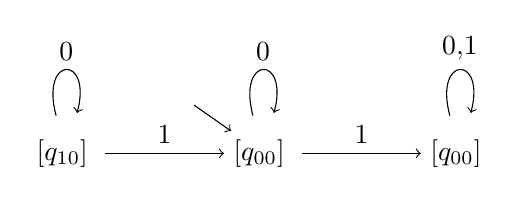
\begin{tikzpicture}
                \node (start) at (-1.5,1.7) {};
                \node (q0) [circle] at (-3,1) {\hspace*{-1mm}$[q_{10}]$};
                \node (q1) [circle,double] at (-0.5,1) {\hspace*{-1mm}$[q_{00}]$};
                \node (q2) [circle] at (2,1) {\hspace*{-1mm}$[q_{00}]$};
                \draw [->] (start) edge (q1);
                \draw [->] (q0) edge[loop above] node {0} (q0);
                \draw [->] (q1) edge[loop above] node {0} (q1);
                \draw [->] (q2) edge[loop above] node {0,1} (q2);
                \draw [->] (q0) edge node [auto] {1} (q1);
                \draw [->] (q1) edge node [auto] {1} (q2);
            \qedhere
        \end{tikzpicture}
\end{center}
\end{Bsp}



\begin{Satz}[name={[Äquivalenzklassenautomat ist wohldefiniert]}]
        Der Äquivalenzklassenautomat ist wohldefiniert und $L(\A_\equiv)=L(\A)$.
\end{Satz}


\begin{proof}\ 
        \begin{enumerate}
                \item Wohldefiniert: Es gilt zu zeigen, dass $\delta_\equiv([q],a) =[\delta(q,a)]$ nicht abhängig von der Wahl des Repräsentanten $q\in [q]$ ist. Dies folgt direkt aus \autoref{eqn:delta-wohldefiniert}.
                \item $L(\A)=L(\A_\equiv)$:
                Zunächst zeigen wir via Induktion über die Länge von $w$, dass für alle $w\in\Sigma^*$ und alle $q\in Q$ die folgende Äquivalenz gilt.
                \[\tilde\delta(q,w)\in F \<=> \tilde\delta_\equiv([q],w)\in F_\equiv\]
                
                
                I.A. $(n=0,$ also $w=\Eps)$: $\tilde\delta(q,\Eps)=q\in F \<=> \tilde\delta_\equiv([q],\Eps)=[q]\in F_\equiv$\\
                I.S.: ($n\rightsquigarrow n+1$) \begin{align*}
                \tilde\delta(q,aw)\in F &\<==> \tilde\delta(\delta(q,a),w)\in F\\ &\xLeftrightarrow{I.V.} \tilde\delta_\equiv([\delta(q,a)],w)\in F_\equiv\\
                &\<==> \tilde\delta_\equiv(\delta_\equiv([q],a),w)\in F_\equiv\\
                &\<==> \tilde\delta_\equiv([q],a w)\in F_\equiv
                \end{align*}
                Mir Hilfe dessen zeigen wir nun $L(\A)=L(\A_\equiv)$. Sei $w\in\Sigma^*$.
                \begin{align*}
                 w\in L(\A)
                 & \<==> \tilde\delta(\qinit,w) \in F\\
                 & \<==> \tilde\delta_\equiv([\qinit],w) \in F_\equiv\\
                 & \<==> w\in L(\A_\equiv)
                 \qedhere
                \end{align*}
        \end{enumerate}
\end{proof}
In den Übungen werden wir ein Verfahren mit Laufzeit $O(|Q|^4\cdot |\Sigma|\log|Q|)$ zur Konstruktion des Äquivalenzklassenautomaten kennenlernen. Es gibt aber auch schnellere Verfahren. Mit dem Algorithmus von Hopcroft kann $\A_\equiv$ in $O(|Q||\Sigma|\log|Q|)$ erzeugt werden.

Wir werden später (\-> Satz von Myhill-Nerode) sehen, dass $\A_\equiv$ der kleinste \acs*{DEA} ist, der $L(\A)$ akzeptiert.

\begin{Def}[name={[Rechtskongruente Äquivalenzrelation]}]
        \datenote{27.10.17}
        Eine Äquivalenzrelation $R\subseteq\Sigma^*\x\Sigma^*$ heißt \emph{rechtskongruent}, falls
        \[
        (u,v)\in R \quad\=>\quad \forall w\in\Sigma^*: (u\cdot w,v\cdot w) \in R.
        \qedhere
        \]
\end{Def}
%\setcounter{Bsp}{5}
\begin{Bsp} %\rlnote{Bsp.-Num. überprüfen (3.6)}
  \label{Bsp:R_m}
        Für einen \ac{DEA} $\A$ definiere
        \[ R_\A = \{(u,v) \mid \tilde\delta(\qinit,u)=\tilde\delta(\qinit,v)\}. \]
        \begin{description}
                \item[Beobachtung 1] $R_\A$ ist eine Äquivalenzrelation.
                
                Dies folgt daraus, dass "`="' eine Äquivalenzrelation ist.
                \item[Beobachtung 2] $R_\A$ ist rechtskongruent. 
                
                Dies wird in den Übungen bewiesen.
                \item[Beobachtung 3] Wir haben pro Zustand, der von $\qinit$ erreichbar ist, genau eine Äquivalenzklasse.
                Der Index von $R_\A$ ist also die Anzahl der erreichbaren Zustände.
        \end{description}
        
        \medskip
        
        Für den \ac{DEA} aus \autoref{bsp:2.schnitt} hat $R_\A$ die folgenden Äquivalenzklassen.
        \begin{align*}
        [\Eps] &= \{0^n\mid n\in \N\}\\
        [1] &= \{0^n10^m\mid n,m\in \N\}\\
        [11] &= \{w\mid \text{Anzahl von Einsen in $w$ ist gerade und $\geq 2$}\}\\
        [111] &= \{w\mid \text{Anzahl von Einsen in $w$ ist ungerade und $\geq 2$}\}
        \qedhere
        \end{align*}
\end{Bsp}
\begin{Def}
        Für eine Sprache $L\subseteq \Sigma^*$ ist die \emph{Nerode-Relation} wie folgt definiert.
        \[
        R_L = \{(u,v) \mid \forall w\in\Sigma^*: uw\in L \<=> vw\in L \}
        \qedhere
        \]
\end{Def}
\begin{description}
 \item[Beobachtung 1] Die Nerode-Relation ist eine Äquivalenzrelation.
 
 Dies folgt daraus, dass "`$\Leftrightarrow$"' (Biimplikation, "`genau dann, wenn"') eine Äquivalenzrelation ist.
 \item[Beobachtung 2] Die Nerode-Relation ist rechtskongruent.
                \begin{proof}
                Sei $(u,v)\in R_L$. Zeige $\forall w\in\Sigma^*: (uw,vw)\in R_L$.
                Wir führen diesen Beweis via Induktion über die Länge von $w$.\\
                I.A. ($n=0$) Für $w=\Eps$ ist $ (u\Eps,v\Eps)=(u,v)\in R_L$.\\
%                 I.S. Sei Aussage gezeigt für alle Wörter $w'$ mit $|w'| \le k$.\\
                I.S. ($n\rightsquigarrow n+1$) Betrachte mit $w=w'a$ ein beliebiges Wort der Länge $n$.
                Nach Induktionsvoraussetzung ist dann auch $(uw', vw') \in R_L $.
                \begin{eqnarray*}
		(uw',vw')\in R_L 
		& \stackrel{\text{Def.\ } R_L}{\text{gdw}} & \forall z\in\Sigma^*: uw'z\in L \<=> vw'z\in L\\
		& \stackrel{\text{zerlege } z=az'}{\text{impliziert}} & \forall a\in \Sigma, z'\in\Sigma^*: uw'az'\in L \<=> vw'az'\in L\\
		& \stackrel{\text{Def.\ } R_L}{\text{impliziert}} & (uw'a,vw'a)\in R_L
		\qedherefixeqnarray
	      \end{eqnarray*}
              \end{proof}
\end{description}

\begin{Bsp}
Sei $\Sigma=\{0,1\}$. Die Sprache $L=\{w\in\Sigma^*\mid \text{vorletztes Zeichen von $w$ ist } 1\}$ hat die folgenden Äquivalenzklassen bezüglich der Nerode-Relation.
        \begin{align*}
        [\Eps] &= \{w\mid w \text{ endet mit } 00 \} \cup \{\varepsilon, 0\}\\
        [1] &= \{w\mid w \text{ endet mit } 01 \} \cup \{1\}\\
        [10] &= \{w\mid w \text{ endet mit } 10 \}\\
        [11] &= \{w\mid w \text{ endet mit } 11 \}
        \qedhere
        \end{align*}
\end{Bsp}

\begin{Bsp}
      Für ein beliebiges Alphabet $\Sigma$ gilt:
      \begin{enumerate}
       \item Die Sprache $L=\{\Eps\}$ hat genau zwei Äquivalenzklassen bezüglich der Nerode-Relation.
      Eine Äquivalenzklasse ist $\{\Eps\}$, die andere ist $\Sigma^+$.
       \item Die Sprache $L=\{\}$ hat genau eine Äquivalenzklasse (nämlich $\Sigma^*$) bezüglich der Nerode-Relation.
       \qedhere
      \end{enumerate}
\end{Bsp}

\begin{Bsp}
Sei $\Sigma=\{0,1\}$. Die Sprache $L_\text{centered}=\{0^n10^n \mid n\in\N\}$ hat bezüglich der Nerode-Relation die folgende Menge von Äquivalenzklassen:
$$\{ [w'] \mid w' \text{ ist Präfix eines Worts } w\in L_\text{centered}\} \cup \{ [11] \}$$
Dabei gilt, dass für je zwei verschiedene $k\in\N$
auch die Äquivalenzklassen $[0^k1]$ verschieden sind. Somit gibt es unendlich viele Äquivalenzklassen.

Bemerkung: Die Äquivalenzklasse $[11]$ enthält alle Wörter, die kein Präfix eines Worts aus $L_\text{centered}$ sind.
\end{Bsp}

% Beispiel: Drei Sprachen $L_a, L_b$ und $L_c$ mit unterschiedlichem Index  (Anzahl an Äquivalenzklassen) bzgl. der Nerode-Relation:
% \begin{alignat*}{2}
%         &\begin{rcases}
%         L_a=\{\Eps\} & [\Eps]\equiv[\Eps]\\
%         w,v\in\Sigma^*,\ w,v\ne\Eps & [w]=[v]
%         \end{rcases} &\ &\text{Index}= 2\\
%         &L_b = \varnothing, L_c= \Sigma^* &&\text{Index}= 1
% \end{alignat*}
% Die Menge der Äquivalenzklassen der Nerode-Relation $R_{L_a}$ auf $L_a$ ist
% \[ L_a / R_{L_a} = \{ [\Eps], [w] \} \]

\begin{Satz}[Myhill und Nerode] % 3.4
        Die folgenden Aussagen sind äquivalent:
        \begin{enumerate}
                \item\label{itm:Nerode1} $L\subseteq \Sigma^*$ wird von einem \ac{DEA} akzeptiert.
                \item\label{itm:Nerode2} $L$ ist Vereinigung die von Äquivalenzklassen einer rechtskongruenten Äquivalenzrelation mit \emph{endlichem} Index.
                \item\label{itm:Nerode3} Die Nerode-Relation $R_L$ hat \emph{endlichen} Index.
                \qedhere
        \end{enumerate}
\end{Satz}

% \datenote{2.11.16}
\begin{proof}
  Wir beweisen die paarweise Äquivalenz in drei Schritten:

  \begin{center}
    (1) \=> (2), \quad \mbox{(2) \=> (3)}\quad \text{und} \quad (3) \=> (1)
  \end{center}

        \paragraph{(1) \=> (2)} Sei $\A$ ein \ac{DEA} mit
  \begin{displaymath}
    L(\A)=\{w \mid \tilde\delta(\qinit,w)\in F \} = \bigcup_{q \in F} \{ w \mid \tilde\delta(\qinit,w) = q\}.
\end{displaymath}
%
Nun sind $\{ w \mid \tilde\delta(\qinit,w)=q \} = [q]_\A$ genau die Äquivalenzklassen der Relation $R_\A$ aus \autoref{Bsp:R_m}, einer rechtskongruenten Äquivalenzrelation.
Der Index ist die Anzahl der erreichbaren Zustände und somit endlich: $\operatorname{\operatorname{Index}}(R_\A) \le |Q| < \infty$.
        
\paragraph{(2) \=> (3)} Sei $R$ einer rechtskongruente Äquivalenzrelation mit endlichem Index, sodass $L$ die Vereinigung von $R$-Äquivalenzklassen ist.
        
Es genügt zu zeigen, dass die Nerode-Relation $R_L$ eine Obermenge von $R$ ist.%
\footnote{
Zur Erklärung: Falls $R \subseteq R_L$, dann gilt $\operatorname{Index}(R) \ge \operatorname{Index}(R_L)$.
Intuitiv: Je mehr Elemente eine Äquivalenzrelation $R$ enthält, desto mehr Elemente sind bzgl.\ dieser Relation äquivalent, d.h.\ desto weniger unterschiedliche Äquivalenzklassen gibt es.
}
\begin{comment}
% Ausformulierter Beweis
Es folgt $u \in L \Leftrightarrow v \in L$, da $L$ aus Vereinigung von Äquivalenzklassen besteht. Da $R$ rechtskongruent ist, folgt für alle $w$:
\[ uw \in L \Leftrightarrow vw \in L \]
Das aber ist die Definition der Nerode-Relation, d.h.\ $(u, v) \in R_L$. Da wir $(u, v)$ beliebig gewählt haben, gilt somit: 
\[\text{\#Klassen($R_L$) $\leq$ \#Klassen($R$)}<\infty\]
\end{comment}
\begin{align*}
(u, v) \in R & \quad\Rightarrow\quad u \in L \Leftrightarrow v \in L \text{, \quad da $L$ Vereinigung von Äquivalenzklassen ist} \\
& \quad\Rightarrow\quad \forall w \in \Sigma^*: uw \in L \Leftrightarrow vw \in L \text{, \quad da $R$ rechtskongruent } \\
& \quad\Rightarrow\quad (u, v) \in R_L \text{, \quad nach Definition der Nerode-Relation}
\end{align*}
Es gilt also $R \subseteq R_L$ und somit $\operatorname{Index}(R_L) \leq \operatorname{Index}(R)<\infty$.


\paragraph{(3) \=> (1)} Gegeben $R_L$, konstruiere $\A=(Q,\Sigma,\delta,\qinit,F)$
    \begin{itemize}
    \item $Q = \{ [w]_{R_L} \mid w\in \Sigma^* \}$ \quad endlich, da $\operatorname{Index}$($R_L$) endlich
    \item $\delta([w],a) = [wa]$ \quad wohldefiniert, da $R_L$ rechtskongruent
    \item $\qinit = [\Eps]$
    \item $F = \{ [w] \mid w\in L \}$
    \end{itemize}
    Wir wollen nun $L(\A)=L$ zeigen. Dafür beweisen wir zunächst via Induktion über die Länge von $w$ die folgende Eigenschaft.
        \begin{displaymath}
      \forall w\in\Sigma^* :
                        \forall v\in\Sigma^* : \tilde\delta([v],w) = [v\cdot w]
    \end{displaymath}
    I.A. $(w = \Eps)$: $\tilde\delta([v],\Eps) = [v]=[v\cdot\Eps]$
    
    I.S. Sei $w = aw'$ beliebiges Wort der Länge $n+1$.
      \begin{displaymath}
        \begin{array}{lcl}
        \tilde\delta([v],aw') &=& \tilde\delta(\delta([v],a),w') \\
                             &=& \tilde\delta([v\cdot a],w') \\
                             &\stackrel{\text{I.V.}}{=}&[v\cdot a\cdot w'] \\
                             &=& [v\cdot \underbrace{aw'}_{=w}]
        \end{array}
      \end{displaymath}

Nun zeigen wir $L(\A)=L$ wie folgt:
\begin{eqnarray*}
        w\in L(\A)
        & \text{gdw} & \tilde\delta([\Eps],w)\in F\\
        & \text{gdw} & [w]\in F, \quad \text{(via Induktion gezeigte Eigenschaft für $v=\Eps$)}\\
        & \text{gdw} & w\in L
        \qedherefixeqnarray
\end{eqnarray*}
\end{proof}
%
\setcounter{Korollar}{4}
\begin{Korollar}\label{kor:2.minAutomat}\datenote{3.11.16}
        Der im Beweisschritt (3) \=> (1) konstruierte Automat $\A$ ist ein minimaler Automat (bzgl.\ der Zustandsanzahl) für eine reguläre Sprache $L$.
\end{Korollar}
\begin{proof}
        Sei $\A'$ ein \emph{beliebiger} \ac{DEA} mit $L(\A')=L$.
        
        Aus "`\ref{itm:Nerode1} {\=>} \ref{itm:Nerode2}"' wissen wir, dass $\operatorname{Index}(R_{\A'})\leq |Q'|$ gilt.
        
        Aus "`\ref{itm:Nerode2} \=> \ref{itm:Nerode3}"' wissen wir, dass $R_{\A'}\subseteq R_L$ und somit $\operatorname{Index}(R_L) \leq \operatorname{Index}(R_{\A'})$ gilt.
        
        In "`\ref{itm:Nerode3} \=> \ref{itm:Nerode1}"' definieren wir $A$, sodass $|Q|=\operatorname{Index}(R_L) \leq \operatorname{Index}(R_\A)\leq |Q'|$ gilt.
        
        Für einen beliebigen \acs*{DEA} $A'$ ist $|Q|$ also nie größer als $|Q'|$.
\end{proof}


\subsection{\acf{PL} für reguläre Sprachen} %\rlnote{subsection \# (3.3)?}
% \datenote{26.10.16 (Eingeschoben)}
Welche interessanten Eigenschaften haben reguläre Sprachen?

Notation: Sei $\operatorname{bin}:\{0,1\}^*\rightarrow \N$ die Decodierung von Bitstrings in natürliche Zahlen;
z.B.\ $\operatorname{bin}(101) = 5$, $\operatorname{bin}(\Eps) = 0$.

\begin{Bsp*} Betrachte den folgenden \ac{DEA}, der die Sprache der Binärcodierung von durch drei teilbaren Zahlen akzeptiert:
                $L = \{ w\in \{0,1\}^* \mid \operatorname{bin}(w)\equiv_3 0\}$
    \begin{center}
                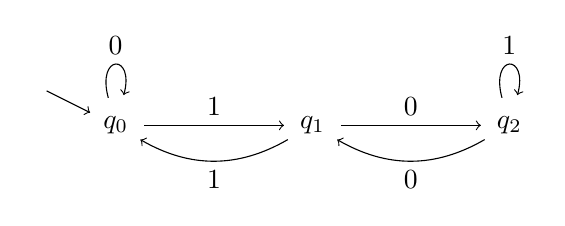
\begin{tikzpicture}
                        \node (start) at (-4,1.5) {};
                        \node (q0) [circle, double] at (-3,1) {$q_0$};
                        \node (q1) [circle] at (-0.5,1) {$q_1$};
                        \node (q2) [circle] at (2,1) {$q_2$};
                        \draw [->] (start) edge (q0);
                        \draw [->] (q0) edge [loop above] node {0} (q0);
                        \draw [->] (q0) edge node [auto] {1} (q1);
                        \draw [->] (q1) edge [bend left] node [auto] {1} (q0);
                        \draw [->] (q1) edge node [auto] {0} (q2);
                        \draw [->] (q2) edge [bend left] node [auto] {0} (q1);
                        \draw [->] (q2) edge [loop above] node {1} (q2);
                \end{tikzpicture}
  \end{center}
  Beobachtungen:
  \begin{itemize}
  \item Es gilt offensichtlich, dass $11 \in L$.
  \item Es gilt auch, dass $1 \underline{0 0} 1 \in L$.
  \item Der Automat hat eine Schleife bei $\tilde\delta({q_1,00}) = q_1$, die mehrfach "`abgelaufen"' werden kann, ohne die Akzeptanz zu beeinflussen.
  \item Also gilt auch $100001 \in L$.
  \item Im Allgemeinen gilt $\forall i\in\N: 1(00)^i1 \in L$.
  \qedhere
  \end{itemize}
\end{Bsp*}
Verdacht: Alle "`langen"' Wörter lassen sich in der Mitte "`aufpumpen"'.
Wir formalisieren diesen Verdacht im folgenden Lemma.

\begin{lemma}[Pumping Lemma]\label{lem:pumping}
        Sei $L$ eine reguläre Sprache. Dann gilt:
        \begin{alignat*}{2}
                &\exists n\in\N,\ n>0:\quad \forall z\in L,\ |z|\geq n:\\
                &\exists u,v,w\in\Sigma^* :\\
                &z = uvw,\ |uv| \leq n,\ |v| \geq 1\\
                \text{und }& \forall i\in\N: uv^iw\in L
        \end{alignat*}
\end{lemma}
\vspace{-2em}
\begin{proof}
	Sei $\A=(\Sigma, Q,\delta,\qinit,F)$ ein beliebiger \ac{DEA} für $L$.
	Wähle $n=|Q|$ und $z\in L$ beliebig mit $|z|\geq n$.
	
	\vspace{-1em}
	
	Beim Lesen von $z$ durchläuft $\A$ genau $\overbrace{|z|+1}^{\geq\; n+1}$ Zustände.
	Somit gibt es mindestens einen Zustand $q\in Q$, der mehrmals besucht wird (Schubfachprinzip).
	
	Wähle den Zustand $q$, der als Erster zweimal besucht wird.
	\begin{alignat*}{3}
		\text{Nun gilt: }\quad
		\exists u:\; && \tilde\delta(\qinit,u)&=q &\qquad& u\text{ Präfix von }z\\
		\exists v:\; && \tilde\delta(q,v)&=q && uv\text{ Präfix von }z\\
		\exists w:\; && \tilde\delta(q,w)&\in F && uvw=z\\
		&& |v| &\geq 1\\
		&& |uv| &\leq n && \text{da $q$ als Erster zweimal besucht wird}
	\end{alignat*}
	\begin{alignat*}{2}
		\text{Es folgt für beliebiges $i\in\N$ :}\quad \tilde\delta(\qinit,uv^iw) &= \tilde\delta(q,v^iw)\\
		&= \tilde\delta(q,w) &\qquad& \text{denn }\forall i: \tilde\delta(q,v^i)=q\\
		&\in F
		\qedherefixalignat
	\end{alignat*}
\end{proof}


\begin{Bsp*}
        Die Sprache $L_\text{centered}=\{0^n10^n \mid n\in\N\}$ ist nicht regulär.
        
        Wir geben hierfür einen Widerspruchsbeweis mit Hilfe des Pumping Lemmas \ac{PL}.
        
        Sei $n$ die Konstante aus dem \ac{PL}. Wähle $z=0^n10^n$. 
        (Gültige Wahl, da $|z|=2n+1\geq n$)\\
        Laut PL existieren $u$, $v$, $w$, sodass $z=uvw$ mit $|v|\geq 1, |uv|\leq n$ und $\forall i \in \N: uv^iw \in L$. 
        Nach Wahl von $z$ gilt nun
  \begin{itemize}
  \item $uv = 0^m$ mit $m\leq n$
  \item $v = 0^k$ mit $k\geq 1$
  \item $w = 0^{n-m}10^n$ 
  \end{itemize}
  Betrachte $uv^2w = 0^{m-k}0^{2k}0^{n-m}10^n = 0^{n+k}10^n \notin L$. Widerspruch!
  Somit ist $L$ nicht regulär.
  
  Zur Illustration:
  \begin{gather*}
    \underbrace{0\ \dots\dots\ 0}_{n} 1 \underbrace{0\ \dots\dots\ 0}_{n}\\
    |\!\ruleplaceholder[u]{\widthof{0\ \dots }} \!|\! \ruleplaceholder[v]{\widthof{\dots 0}}\!|% 
    \ruleplaceholder[w]{\widthof{\ \ \ $1\ \dots\dots\ 1$}}\!|
    \qedhere
  \end{gather*}
\end{Bsp*}

% \begin{Bsp*}
%         $L=\{0^{x^2} \mid x\in\N\}$ ist nicht regulär.\\
%         Sei $n$ die Konstante aus dem \ac{PL}.
%         
%         Wähle $z=0^{n^2}$. Also $|z|=n^2\geq n$\\
%         Laut PL existieren $u$, $v$, $w$, sodass $z=uvw$ mit $|v|\geq 1, |uv|\leq n$ und $\forall i \in \N: uv^iw \in L$. Nach Wahl von $z$ gilt nun
%   \begin{itemize}
%   \item $uv = 0^m$ mit $m\leq n$
%   \item $v = 0^k$ mit $k\geq 1$
%   \item $w = 0^{n^2 - m}$ mit $k\geq 1$
%   \end{itemize}
%   Betrachte $uv^2w = uvvw = 0^{m}0^k0^{n^2-m} = 0^{n^2+k}$.
%   Da $n^2+k$ keine Quadratzahl sein kann ist $uv^2w \not \in L$, und somit ist $L$ nicht regulär.
%   Begründung: betrachte $(n+1)^2 - n^2 = n^2 + 2n + 1 - n^2 = 2n + 1$.
%   Aber $k \le m \le n \le 2n + 1$.
% \end{Bsp*}
% 
% \begin{Bsp*}
% $L_2 = \{0^p \mid p\text{ ist Primzahl}\}$ ist nicht regulär.
% 
% Sei $n$ Konst. aus dem \ac{PL}, $p$ Primzahl mit $p \geq n$.\\
% Wähle $z=0^p \in L_2$
% \begin{align*}
%         \ac{PL}:\ &z=uvw \text{ mit } |uv|\leq n &&,|v| \geq 1\\
%         &\curvearrowright |z|= p=a+b &&, a = |uw| \quad, b= |v|\\
%         &\curvearrowright |uv^iw| = a + ib &&, \text{wähle }i=p+1\\
%         &\curvearrowright |uv^{p+1}w| = a + (p+1)b & =& a + pb + b = p+pb \text{ keine Primzahl} \\
%         \text{Also } &uv^{p+1}w \notin L_2\\
%         &\curvearrowright L_2\text{ nicht regulär.}
%   \qedhere
% \end{align*}
% \end{Bsp*}


\subsection[\acf{NEA}]{Nichtdeterministischer endlicher Automat (NEA)}
Aufgabe: Konstruiere für eine natürliche Zahl $n\in\N$ einen \acs*{DEA} für die folgende Sprache.
	\begin{align*}
		L_n &= \{ w\in\{0,1\}^* \mid \text{das $n$-letzte Symbol von $w$ ist 1} \}
	\end{align*}
Naiver Lösungsversuch:
	\begin{figure}[H]\centering
		\begin{tikzpicture}[>=stealth, shorten >=1pt,
				node distance=1.5cm, on grid, initial text=,
				every state/.style={minimum size=0pt,inner sep=0pt}
			]
			\node[state,initial] (q0) {};
			\node[state] (q1) [right of=q0] {};
			\node        (q2) [right of=q1] {\dots};
			\node[state,accepting] (q3) [right of=q2] {};
			\path[->]
				(q0) edge [loop above] node [auto] {$\Sigma$} ()
				     edge              node [auto] {1}        (q1)
				(q1) edge              node [auto] {$\Sigma$} (q2)
				(q2) edge              node [auto] {$\Sigma$} (q3)
			;
			\draw [thick, decoration={brace, mirror, raise=.3cm, amplitude=10pt}, decorate]
			    (q1.west) -- (q3.east)
			    node [pos=0.5,anchor=north,yshift=-0.65cm] {n};
		\end{tikzpicture}
		\caption{Nichtdeterministischer Automat für $L_n$}
		\label{fig:2.nletztesNea}
	\end{figure}
Problem: Das Zustandsdiagramm beschreibt keinen \acs*{DEA}:
Der Startzustand hat zwei ausgehende Kanten für $1$.

Untersuche die Sprache mit Hilfe der Nerode-Relation.
Beobachtung: Je zwei Wörter der Länge $n$ sind in unterschiedlichen Äquivalenzklassen.
Es gibt also mindestens $2^n$ Äquivalenzklassen; aus \autoref{kor:2.minAutomat} wissen wir, dass ein minimaler \acs*{DEA}, der $L_n$ akzeptiert, mindestens $2^n$ Zustände haben muss.

Idee: Definiere einen neue Art von Automaten, bei dem ein Zustand pro Zeichen mehrere Nachfolger haben darf.

% \begin{Bsp*} Mustererkennung\\
% 	kommt ein String (konsistent) in einem anderen vor?
% 	
% 	Gegeben: festes Wort $w$.\\
% 	Gesucht: Sprache aller Worte, in denen $w$ als Teilwort vorkommt.
% 	\begin{align*}
% 		L &= \{ v\in\Sigma^* \mid \exists u,x\in\Sigma^*: v=uwx \}\\
% 		\Sigma &= \{a,b,c\}\\
% 		& \text{konkretes Beispiel:}\\
% 		w &= abac
% 	\end{align*}
% 	\begin{figure}[tp]
% 	\centering
% 		\begin{tikzpicture}[>=stealth, shorten >=1pt,
% 				node distance=2cm, on grid, initial text=,
% 				every state/.style={minimum size=0pt,inner sep=0pt}
% 			]
% 			\node[state,initial] (q0) {};
% 			\node[state] (q1) [right of=q0] {};
% 			\node[state] (q2) [right of=q1] {};
% 			\node[state] (q3) [right of=q2] {};
% 			\node[state,accepting] (q4) [right of=q3] {};
% 			\path[->]
% 				(q0) edge [loop above]    node [auto]  {$b,c$}    ()
% 				     edge                 node [auto]  {$a$}      (q1)
% 				(q1) edge [loop above]    node [auto]  {$a$}      ()
% 				     edge [bend left]     node [auto]  {$c$}      (q0)
% 				     edge                 node [auto]  {$b$}      (q2)
% 				(q2) edge [bend left=50]  node [auto]  {$b,c$}    (q0)
% 				     edge                 node [auto]  {$a$}      (q3)
% 				(q3) edge                 node [auto]  {$c$}      (q4)
% 				     edge [bend right=70] node [above] {$a$}      (q1)
% 				     edge [bend right=40] node [above] {$b$}      (q2)
% 				(q4) edge [loop right]    node [auto]  {$\Sigma$} ()
% 			;
% 		\end{tikzpicture}
% 	\caption{\acs*{DEA} für $L$}
% 	\label{fig:dfa-teilwort}
% 	\end{figure}
% 	\hyperref[fig:dfa-teilwort]{Abbildung~\ref*{fig:dfa-teilwort}} enthält einen \ac{DEA} für die Sprache $L$. Beobachtung: nicht-trivial zu konstruieren.
% 	\begin{figure}[tp]\centering
% 		\begin{tikzpicture}[>=stealth,shorten >=1pt,
% 				node distance=2cm,on grid,
% 				initial text=
% 			]
% 			\node[state,initial] (q0) {$q_0$};
% 			\node[state] (q1) [right of=q0] {$q_1$};
% 			\node[state] (q2) [right of=q1] {$q_2$};
% 			\node[state] (q3) [right of=q2] {$q_3$};
% 			\node[state,accepting] (q4) [right of=q3] {$q_4$};
% 			\path[->]
% 				(q0) edge [loop above] node [auto] {$\Sigma$} ()
% 				     edge              node [auto] {$a$} (q1)
% 				(q1) edge              node [auto] {$b$} (q2)
% 				(q2) edge              node [auto] {$a$} (q3)
% 				(q3) edge              node [auto] {$c$} (q4)
% 				(q4) edge [loop above] node [auto] {$\Sigma$} ()
% 			;
% 		\end{tikzpicture}
% 		\caption{Bsp.: Mustererkennung}
% 		\label{fig:nfa-teilwort}
% 	\end{figure}
% 	
% 	\hyperref[fig:nfa-teilwort]{Abbildung~\ref*{fig:nfa-teilwort}} enthält einen nicht-deterministischen endlichen Automat für die Sprache $L$. Idee: Ein Wort $w$ wird akzeptiert, falls es einen mit $w$ markierten Pfad von $q_0$ zu einen akzeptierenden Zustand gibt.
% 	\begin{figure}[tp]
% 	\centering
% 		\begin{tikzpicture}[>=stealth,shorten >=1pt,
% 				node distance=2cm,on grid
% 			]
% 			\node (q0) {$\{0\}$};
% 			\node (q1) [right of=q0] {$\{0,1\}$};
% 			\node (q2) [right of=q1] {$\{0,2\}$};
% 			\node (q3) [right of=q2] {$\{0,1,3\}$};
% 			\path[->]
% 				(q0) edge [loop below] node [auto] {$b,c$} ()
% 				     edge              node [auto] {$a$} (q1)
% 				(q1) edge [loop below] node [auto] {$a$} ()
% 				(q1) edge              node [auto] {$b$} (q2)
% 				(q2) edge              node [auto] {$a$} (q3)
% 			;
% 		\end{tikzpicture}
% 	\caption{Potenzmengenkonstruktion auf dem \acs*{NEA}}
% 	\label{fig:nfa-teilwort-powerset}
% 	\end{figure}
% 	
% 	\hyperref[fig:nfa-teilwort-powerset]{Abbildung~\ref{fig:nfa-teilwort-powerset}} zeigt (einen Ausschnitt) aus dem deterministischen Automaten, der schematisch aus dem \acsu{NEA} in \autoref{fig:nfa-teilwort} konstruiert werden kann. Idee: bei Schritt mit Symbol $a$ ist der \ac{NEA} gleichzeitig in allen Zuständen, die durch $a$ von (der Menge der) aktuellen Zustände erreichbar sind.
% 	
% 	Variante: erkenne \textbf{Subwort} $w=a_1,\dots,a_n$
% 	\[ L' = \{ v\in\Sigma^* \mid \exists x_0,\dots,x_n\in\Sigma^*: v=x_0a_1x_1a_2\dots a_nx_n \} \]
% 	Nicht det. Automat für $L'$ mit $(w=abac)$ ist sehr einfach. Der entsprechende deterministische Automat ist deutlich komplizierter. (selbst)
% 	\begin{figure}[H]\centering
% 		\begin{tikzpicture}[>=stealth, shorten >=1pt,
% 				node distance=2cm, on grid, initial text=,
% 				every state/.style={minimum size=0pt,inner sep=0pt}
% 			]
% 			\node[state,initial] (q0) {};
% 			\node[state] (q1) [right of=q0] {};
% 			\node[state] (q2) [right of=q1] {};
% 			\node[state] (q3) [right of=q2] {};
% 			\node[state,accepting] (q4) [right of=q3] {};
% 			\path[->]
% 				(q0) edge [loop above] node [auto] {$\Sigma$} ()
% 				     edge              node [auto] {$a$}      (q1)
% 				(q1) edge [loop below] node [auto] {$\Sigma$} ()
% 				     edge              node [auto] {$b$}      (q2)
% 				(q2) edge [loop below] node [auto] {$\Sigma$} ()
% 				     edge              node [auto] {$a$}      (q3)
% 				(q3) edge [loop below] node [auto] {$\Sigma$} ()
% 				     edge              node [auto] {$c$}      (q4)
% 				(q4) edge [loop right] node [auto] {$\Sigma$} ()
% 			;
% 		\end{tikzpicture}
% 		\caption{Nichtdet. Automat für $L'$}
% 	\end{figure}
% 	
% 	Weiteres Beispiel, bei dem der deterministische Automat beweisbar exponentiell größer ist.
% 	\begin{align*}
% 		L_n &= \{ w\in\{0,1\}^* \mid \text{das $n$-letzte Symbol von $w$ ist 1} \}
% 	\end{align*}
% 	\begin{figure}[H]\centering
% 		\begin{tikzpicture}[>=stealth, shorten >=1pt,
% 				node distance=1.5cm, on grid, initial text=,
% 				every state/.style={minimum size=0pt,inner sep=0pt}
% 			]
% 			\node[state,initial] (q0) {};
% 			\node[state] (q1) [right of=q0] {};
% 			\node        (q2) [right of=q1] {\dots};
% 			\node[state,accepting] (q3) [right of=q2] {};
% 			\path[->]
% 				(q0) edge [loop above] node [auto] {$\Sigma$} ()
% 				     edge              node [auto] {1}        (q1)
% 				(q1) edge              node [auto] {$\Sigma$} (q2)
% 				(q2) edge              node [auto] {$\Sigma$} (q3)
% 			;
% 			\draw [thick, decoration={brace, mirror, raise=.3cm, amplitude=10pt}, decorate]
% 			    (q1.west) -- (q3.east)
% 			    node [pos=0.5,anchor=north,yshift=-0.65cm] {n};
% 		\end{tikzpicture}
% 		\caption{Nichtdet. Automat für $L_n$}
% 	\end{figure}
% 	
% 	Der entsprechende deterministische Automat für $L_n$ hat $\sim 2^n$ Zustände.
% \end{Bsp*}

\goodbreak

\begin{Def}[\acs*{NEA}]
        Ein \emph{\acf{NEA}}, (\acsu{NFA} $\hat=$ \acl{NFA}) ist ein 5-Tupel
        \[ \calN= (\Sigma, Q,\delta,\qinit,F). \]
Dabei ist
        \begin{itemize}
                \item $\Sigma$ ein Alphabet,
                \item $Q$ eine \emph{endliche} Menge, deren Elemente wir \emph{Zustände} nennen,
                \item $\delta:Q\x\Sigma\->\mathcal{P}(Q)$ eine Funktion, die wir \emph{Transitionsfunktion} nennen,
                \item $\qinit\in Q$ ein Zustand, den wir \emph{Startzustand} nennen und
                \item $F\subseteq Q$ eine Teilmenge der Zustände, deren Elemente wir \emph{akzeptierende} Zustände nennen.
                \qedhere
        \end{itemize}
\end{Def}
Bemerkung: Die Definition des \acs*{NEA} unterscheidet sich vom \acs*{DEA} also nur in der Transitionsfunktion. Beim \acs*{DEA} ist der Bildbereich der Transitionsfunktion die Menge der Zustände $Q$. Beim \acs*{NEA} ist der Bildbereich die Potenzmenge $\mathcal{P}(Q)$ der Zustandsmenge~$Q$.
Analog zu \acs*{DEA}s werden wir auch \acs*{NEA}s mit Hilfe eines Zustandsdiagramms beschrieben. Zum Beispiel beschreibt \autoref{fig:2.nletztesNea} für jedes $n\in\N$ einen \acs*{NEA} für die Sprache $L_n$.

Im Folgenden sei $\calN$ immer ein \acs*{NEA}.
\begin{Def}[name={[Lauf eines Automaten]}]
	Wir nennen eine Folge von Zuständen $q_0q_1\dots q_n$ einen \emph{Lauf von $\calN$ über $w=a_1\dots a_n$}, falls
	$q_i\in\delta(q_{i-1},a_i)$ für alle $i$ mit $1\leq i\leq n$.
	Wir nennen einen Lauf \emph{initial}, falls $q_0=\qinit$.
	Wir nennen einen Lauf \emph{akzeptierend}, falls $q_n\in F$.
\end{Def}
\datenote{8.11.17}
\begin{Def}[name={[NEA zu DEA]}]
	Ein Wort $w\in\Sigma^*$ wird von $\calN$ \emph{akzeptiert}, falls $\calN$ einen initialen und akzeptierenden Lauf über $w$ hat.
	Die von $\calN$ akzeptierte Sprache ist die Menge der von $\calN$ akzeptierten Wörter, d.h.\
	$L(\calN)=\{ w\in\Sigma^* \mid \exists\text{ initialer, akzeptierender Lauf von $\calN$ über }w \}$.
\end{Def}




\begin{Bsp}
\label{bsp:2.zweitletztes} Der \acs*{NEA} für die Sprache 
$$L_2=\{w\in\{0,1\}^*\mid \text{ das zweitletzte Zeichen von $w$ ist $1$ }\}$$ hat die folgende graphische Repräsentation.
  \begin{center}
                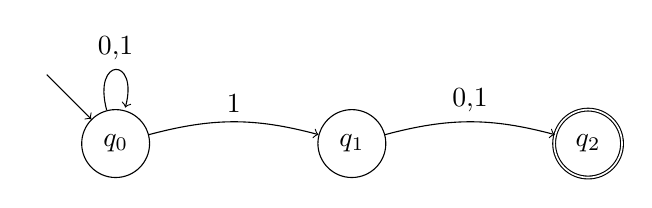
\begin{tikzpicture}[circle/.style={
                        shape=circle,
                        minimum size=0.5cm,
                        text=black, draw,
                        text width=0.5cm,
                        align=center}]
                        \node (vs) at (-1.0,1.0) {};
                        \node [circle] (v0) at (0,0) {$q_{0}$};
                        \node [circle] (v1) at (3,0) {$q_{1}$};
                        \node [circle, double] (v2) at (6,0) {$q_{2}$};
                        \draw [->] (vs) edge (v0);
                        \draw [->] (v0) edge [loop above] node[auto] {0,1} (v2);
                        \draw [->] (v0) edge [bend left=15] node[auto] {1} (v1);
                        \draw [->] (v1) edge [bend left=15] node[auto] {0,1} (v2);
                        \qedhere
                \end{tikzpicture}
  \end{center}
\end{Bsp}


Bemerkung: Die Frage, ob ein gegebenes Wort $w$ akzeptiert wird (das "`Wortproblem"'), lässt sich für \acs*{NEA}s nicht mehr so leicht beantworten wie wir es von \acs*{DEA}s gewohnt sind.
Ein sinnvolles Vorgehen scheint, jeden initialen Lauf zu betrachten, doch z.B.\ für das Wort $111$ hat obiger \acs*{NEA} bereits  drei verschiedene initiale Läufe: $q_0q_0q_0$, $q_0q_0q_1$, $q_0q_0q_2$.


Bemerkung: Die Definitionen von \ac{NEA} und \ac{DEA} in der Literatur sind nicht einheitlich. 
Es gibt äquivalente \ac{NEA}-Definitionen, die statt der Transitionsfunktion $\delta:Q\x\Sigma\->\mathcal{P}(Q)$ eine Transitionsrelation $\delta\subseteq Q\x\Sigma\x Q$ verwenden.
Es gibt alternative \ac{NEA}-Definitionen, die eine Menge von Startzuständen erlauben.
Alternativ könnte man auch zunächst den \ac{NEA} einführen und den \ac{DEA} als Spezialfall dessen definieren (Spezialfall: Das Bild der Transitionsfunktion ist einelementig für alle $q\in Q$ und $a\in\Sigma$).

Bemerkung: Zu jedem \ac{DEA} $\A= (\Sigma, Q,\delta,\qinit,F)$ gibt es einen \ac{NEA}, der die gleiche Sprache akzeptiert.
Beispiel: der \ac{NEA} $\calN= (\Sigma, Q,\delta_\mathsf{NEA},\qinit,F)$ mit $\delta_\mathsf{NEA}(q,a)=\{\delta(q,a)\}$, der sich von $\A$ nur in der Transitionsfunktion unterscheidet.


\begin{Satz}[Rabin und Scott]\label{satz:2.rabinscott}
	Zu jedem \ac{NEA} $\calN$ mit $n$ Zuständen gibt es einen \ac{DEA} $\A_\calP$ mit $2^n$ Zuständen, sodass $L(\A_\calP)=L(\calN)$ gilt.
\end{Satz}
  Zur Vorbereitung des Beweises machen wir zunächst die folgende Definition.

\begin{Def}[Potenzmengenautomat]
 Für einen gegebenen \ac{NEA}  $\calN= (\Sigma, Q,\delta,\qinit,F)$ ist der Potenzmengenautomat $\A_\calP$ wie folgt definiert.
         \begin{align*}
                Q_\calP &= \mathcal{P}(Q)\\
                \delta_\calP(p,a) &= \bigcup_{q\in p} \{\delta(q,a)\}\\
                \qinit_\calP &= \{\qinit\}\\
                F_\calP &= \{ p\in Q_\calP \mid p\cap F\neq \varnothing \}
                \qedhere
        \end{align*}
\end{Def}
\begin{Bsp}
Der Potenzmengenautomat für den \acs*{NEA} aus \autoref{bsp:2.zweitletztes} hat das folgende Zustandsdiagramm.
  \begin{center}
                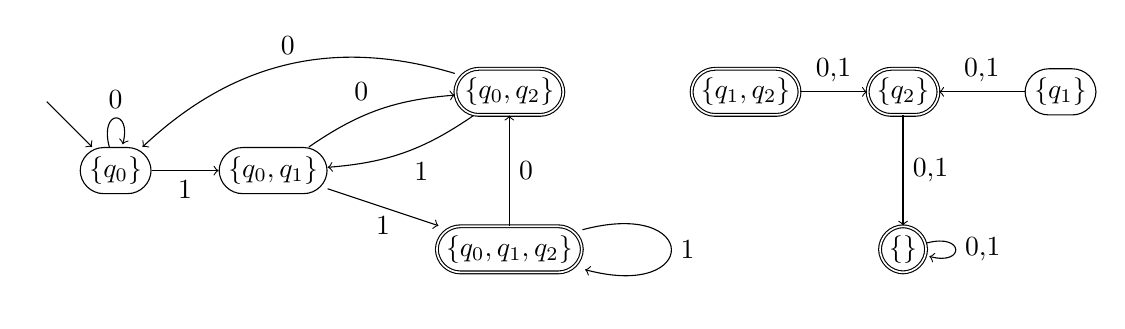
\begin{tikzpicture}[circle/.style={
                        shape=circle,
                        minimum size=0.5cm,
                        text=black, draw,
                        text width=0.5cm,
                        align=center}]
                        \node (vs) at (-1.0,1.0) {};
                        \node [draw, rounded corners=3mm] (v0) at (0,0) {$\{q_{0}\}$};
                        \node [draw, rounded corners=3mm] (v1) at (2,0) {$\{q_{0}, q_1\}$};
                        \node [draw, rounded corners=3mm, double] (v2) at (5,1) {$\{q_0, q_{2}\}$};
                        \node [draw, rounded corners=3mm, double] (v3) at (5,-1) {$\{q_0, q_1, q_2\}$};
                        \node [draw, rounded corners=3mm, double] (v4) at (8,1) {$\{q_1, q_2\}$};
                        \node [draw, rounded corners=3mm] (v5) at (12,1) {$\{q_1\}$};
                        \node [draw, rounded corners=3mm, double] (v6) at (10,1) {$\{q_2\}$};
                        \node [draw, rounded corners=3mm, double] (v7) at (10,-1) {$\{\}$};
                        \draw [->] (vs) edge (v0);
                        \draw [->] (v0) edge [loop above] node[auto] {0} (v2);
                        \draw [->] (v0) edge [bend left=0] node[below] {1} (v1);
                        \draw [->] (v1) edge [bend left=15] node[auto] {0} (v2);
                        \draw [->] (v1) edge [bend left=0] node[below] {1} (v3);
                        \draw [->] (v2) edge [bend right=30] node[above] {0} (v0);
                        \draw [->] (v2) edge [bend left=15] node[auto] {1} (v1);
                        \draw [->] (v3) edge [bend left=0] node[right] {0} (v2);
                        \draw [->] (v3) edge [loop right] node[auto] {1} (v3);
                        \draw [->] (v4) edge [] node[auto] {0,1} (v6);
                        \draw [->] (v5) edge [] node[auto,above] {0,1} (v6);
                        \draw [->] (v6) edge [] node[auto] {0,1} (v7);
                        \draw [->] (v7) edge [loop right] node[auto] {0,1} (v7);
                \end{tikzpicture}
  \end{center}
Die vier Zustände auf der rechten Seite sind nicht erreichbar.
\end{Bsp}


% \draftnote{4.11.16}
\begin{proof}[von \autoref{satz:2.rabinscott}]
        Zeige $L(\A_\calP)=L(\calN)$. 
        Dafür beweisen wir zunächst via Induktion über die Länge von $w$ die folgende Eigenschaft:
        
        $\forall w\in\Sigma^*\; \forall p\in Q_\calP\backslash\{\{\}\}\; \forall q\in Q:$
        $$q\in\tilde\delta_\calP(p,w) \Leftrightarrow \exists \underbrace{q_0, q_1,\ldots, q_n}_{\text{Lauf}}\in Q, \text{ sodass }  n=|w|, q_0\in p \text{ und } q_n=q$$
        I.A. $(n=0,$ also $w=\Eps)$: Gilt trivialerweise, da $p\neq\{\}$.\\
        I.S. ($n\rightsquigarrow n+1$): Sei $w=aw'$ ein beliebiges Wort der Länge $n+1$.
        \begin{eqnarray*}
                q\in\tilde\delta_\calP(p,w) 
                \hspace*{-2.5mm} & \Leftrightarrow & \hspace*{-2.5mm} q\in\tilde\delta_\calP(\delta_\calP(p,a),w')\\
                & \stackrel{\text{I.V.}}{\Leftrightarrow} & \hspace*{-2.5mm} \exists\underbrace{q_1,q_2,\ldots, q_{n+1}}_{\text{Lauf}}\in Q, \text{ sodass }  n=|w'|, q_1\in \delta_\calP(p,a) \text{ und } q_{n+1}=q\\
                & \Leftrightarrow & \hspace*{-2.5mm}\exists\underbrace{q_1,q_2,\ldots, q_{n+1}}_{\text{Lauf}}\in Q, \text{ sodass }  n=|w'|, \exists q_0\in p: q_1\in\delta(q_0,a) \text{ und } q_{n+1}=q\\
                & \Leftrightarrow & \hspace*{-2.5mm} \exists\underbrace{q_0,q_1,q_2,\ldots, q_{n+1}}_{\text{Lauf}}\in Q,\text{ sodass }  n+1=|w|, q_0\in p \text{ und } q_{n+1}=q
        \end{eqnarray*}
        Mit Hilfe dieser Eigenschaft zeigen wir nun die Gleichheit $L(\A_\calP)=L(\calN)$.
        \begin{align*}
         w\in L(\A_\calP) 
         &\<=> \tilde\delta_\calP(\qinit_\calP,w)\in F_\calP\\
         &\<=> \exists q_f\in \tilde\delta_\calP(\qinit_\calP,w)\cap F\\
         &\<=> \exists \underbrace{q_0, q_1,\ldots, q_n}_{\text{Lauf}}\in Q, \text{ sodass }  n=|w|, q_0\in \qinit \text{ und } q_n\in F\\
         &\<=> \exists \text{ initialer, akzeptierender Lauf von $\calN$ über $w$} \\
         &\<=> w\in L(\calN)
         \qedhere
        \end{align*}
\end{proof}

Bemerkung: Es gelten also die folgenden Äquivalenzen.
\[
L \text{ regulär} 
\ \ \stackrel{\text{\autoref{def:2.sprache}}}{\Longleftrightarrow} \ \ L = L(\A) \text{ für einen \ac{DEA} }\A
\ \ \Longleftrightarrow \ \ L = L(\calN) \text{ für einen \ac{NEA} }\calN
\]
Bemerkung: \ac{NEA}s sind eine exponentiell kompaktere Repräsentation von regulären Sprachen im folgenden Sinne:
\begin{enumerate}
 \item Es gibt mit $L_n$ ($n$-letztes Zeichen) eine Menge von Sprachen, die sich durch einen \ac{NEA} mit $n+1$ Zuständen darstellen lassen, aber bei denen ein minimaler \ac{DEA} mindestens $2^n$ Zustände hat. (Siehe Übungsblatt 3, Aufgabe 2).
 \item Zu jedem \ac{NEA} mit $n$ Zuständen gibt es einen \ac{DEA} mit $2^n$ Zuständen, der die gleiche Sprache akzeptiert. (\autoref{satz:2.rabinscott}).
 \item Zu jedem \ac{DEA} mit $n$ Zuständen gibt es einen \ac{NEA} mit $n$ Zuständen, der die gleiche Sprache akzeptiert.
\end{enumerate}

\subsubsection{\texorpdfstring{$\Eps$}{epsilon}-Übergänge}\label{sec:2.EpsNea}
In diesem Unterkapitel führen wir mit dem $\Eps$-NEA ein weiteres Automatenmodell ein. 
Wir wollen $\Eps$-NEAs zunächst durch die folgende Fragestellung und anschließende Diskussion motivieren.

Frage: Gegeben zwei reguläre Sprachen $L_1, L_2$, ist auch die Konkatenation $L_1\cdot L_2$ eine reguläre Sprache?

Idee: Gegeben \acs*{DEA} $\A_1$ mit $L(\A_1)=L_1$ und \acs*{DEA} $\A_2$ mit $L(\A_2)=L_2$,
konstruiere \acs*{NEA} für $L_1\cdot L_2$ durch "`Hintereinanderschalten"' von $\A_1$ und $\A_2$;
immer wenn wir in einem akzeptierenden Zustand von $\A_1$ sind, erlauben wir, in $\A_2$ zu "`wechseln"'.

Erste, naive (und inkorrekte) Umsetzung dieser Idee: 
Verschmelze akzeptierende Zustände von $\A_1$ mit dem Startzustand von $\A_2$
Wir betrachten die folgenden Automaten, um zu sehen, dass diese Umsetzung nicht zielführend ist.
\definecolor{auto1}{RGB}{200,200,255}
\definecolor{auto2}{RGB}{255,100,100}
\begin{Bsp}\label{bsp:2.naiveconcat}
Links: \acs*{DEA} $\A_1$, der Automat aus \autoref{bsp:2.zweitletztes} eingeschränkt auf die erreichbaren Zustände. Rechts: \acs*{DEA} $\A_2$ mit der Sprache $\{w\in\{0,1\}^*\mid \text{Anzahl $1$ in $w$ ungerade}\}$.
  \begin{center}
                \begin{tikzpicture}[circle/.style={
                        shape=circle,
                        minimum size=0.5cm,
                        text=black, draw,
                        text width=0.5cm,
                        align=center}]
                        \node (vs) at (-1.0,1.0) {};
                        \node [circle, fill=auto1] (v0) at (0,0) {$p_0$};
                        \node [circle, fill=auto1] (v1) at (2,0) {$p_1$};
                        \node [circle, fill=auto1, accepting, thick] (v2) at (5,1) {$p_2$};
                        \node [circle, fill=auto1, accepting, thick] (v3) at (5,-1) {$p_3$};
                        \draw [->] (vs) edge (v0);
                        \draw [->] (v0) edge [loop above] node[auto] {0} (v2);
                        \draw [->] (v0) edge [bend left=0] node[below] {1} (v1);
                        \draw [->] (v1) edge [bend left=15] node[auto] {0} (v2);
                        \draw [->] (v1) edge [bend left=0] node[below] {1} (v3);
                        \draw [->] (v2) edge [bend right=30] node[above] {0} (v0);
                        \draw [->] (v2) edge [bend left=15] node[auto] {1} (v1);
                        \draw [->] (v3) edge [bend left=0] node[right] {0} (v2);
                        \draw [->] (v3) edge [loop right] node[auto] {1} (v3);
                \end{tikzpicture}
                \quad
                \begin{tikzpicture}[circle/.style={
                        shape=circle,
                        minimum size=0.5cm,
                        text=black, draw,
                        text width=0.5cm,
                        align=center}]
                        \node (ss) at (-1.0,1.0) {};
                        \node [circle, fill=auto2] (s0) at (0,0) {$s_0$};
                        \node [circle, fill=auto2, accepting, thick] (s1) at (3,0) {$s_1$};
                        \draw [->] (ss) edge (s0);
                        \draw [->] (s0) edge [loop above] node[auto] {0} (s0);
                        \draw [->] (s1) edge [loop above] node[auto] {0} (s1);
                        \draw [->] (s0) edge [bend left=15] node[auto] {1} (s1);
                        \draw [->] (s1) edge [bend left=15] node[auto] {1} (s0);
                \end{tikzpicture}
  \end{center}
Unten: \acs*{NEA} $\calN_\mathsf{naiv}$ aus der naiven und inkorrekten Konstruktion für die Konkatenation.
  \begin{center}
                \begin{tikzpicture}[circle/.style={
                        shape=circle,
                        minimum size=0.5cm,
                        text=black, draw,
                        text width=0.5cm,
                        align=center}]
                        \node (vs) at (-1.0,1.0) {};
                        \node [circle, fill=auto1] (v0) at (0,0) {$p_0$};
                        \node [circle, fill=auto1] (v1) at (2,0) {$p_1$};
                        \node [circle, fill=auto1!50!auto2] (v2) at (5,1.5) {\hspace*{-1mm}$p_2s_0$};
                        \node [circle, fill=auto1!50!auto2] (v3) at (5,-1.5) {\hspace*{-1mm}$p_3s_0$};
                        \draw [->] (vs) edge (v0);
                        \draw [->] (v0) edge [loop above] node[auto] {0} (v2);
                        \draw [->] (v0) edge [bend left=0] node[below] {1} (v1);
                        \draw [->] (v1) edge [bend left=15] node[auto] {0} (v2);
                        \draw [->] (v1) edge [bend left=0] node[below] {1} (v3);
                        \draw [->] (v2) edge [bend right=30] node[above] {0} (v0);
                        \draw [->] (v2) edge [bend left=15] node[auto] {1} (v1);
                        \draw [->] (v3) edge [bend left=0] node[right] {0} (v2);
                        \draw [->] (v3) edge [loop below] node[auto] {1,0} (v3);
                        \node [circle, fill=auto2, accepting, thick] (va) at (8,0) {$s_1$};
                        \draw [->] (va) edge [loop above] node[auto] {0} (va);
                        \draw [->] (v2) edge [bend left=15] node[auto] {1} (va);
                        \draw [->] (va) edge [bend left=0] node[auto] {1} (v2);
                        \draw [->] (v3) edge [bend left=0] node[auto] {1} (va);
                        \draw [->] (va) edge [bend left=15] node[auto] {1} (v3);
                        \draw [->] (v2) edge [loop above] node[auto] {0} (v2);
                \end{tikzpicture}
  \end{center}
Dieser \acs*{NEA} akzeptiert nun auch das Wort $w=11011$. Allerdings ist $w$ nicht in der Konkatenation $L(\A_1)\cdot L(\A_2)$, denn es gibt keine Zerlegung $w=w_1\cdot w_2$, sodass sowohl das Präfix $w_1$ von $\A_1$ als auch das Suffix $w_2$ von $\A_2$ akzeptiert wird.
\end{Bsp}


Das "`Verschmelzen"' von $p_2$ (bzw.\ $p_3$) mit $s_0$ war also keine gute Idee.
Was uns aber helfen würde: ein Zustandsübergang, der es uns erlaubt, von Zustand $p_2$ (bzw.\ $p_3$) in den Zustand $s_0$ zu gehen, ohne dabei ein Zeichen zu lesen.

Wir nennen solch einen Zustandsübergang $\Eps$-Übergang und definieren einen Automaten, der solche Zustandsübergänge haben kann, wie folgt.

\begin{Def}[$\Eps$-NEA]\label{def2.EpsNea}
        Ein \emph{nichtdeterministischer endlicher Automat mit $\Eps$-Übergängen} ist ein 5-Tupel
        \[ \B= (\Sigma, Q,\delta,\qinit,F) \]
wobei $\Sigma$, $Q$, $\qinit$, $F$ wie bei \acs*{NEA}s (bzw.\ \acs*{DEA}s) definiert sind und die Transitionsfunktion den folgenden Typ hat.
\[
\delta:Q\x(\Sigma\cup\{\Eps\})\->\mathcal{P}(Q)
\qedhere
\]
\end{Def}

\begin{Bsp}\label{bsp2.EpsNeaEx} 
   \datenote{10.11.17}
   Zustandsdiagramm eines $\Eps$-NEA über dem Alphabet $\Sigma=\{a,b\}$.
   \begin{center}
                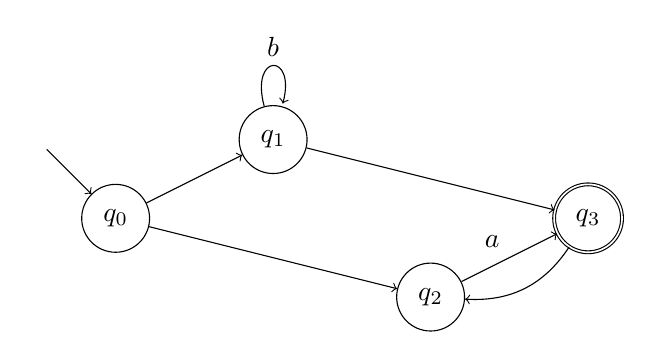
\begin{tikzpicture}[circle/.style={
                        shape=circle,
                        minimum size=0.5cm,
                        text=black, draw,
                        text width=0.5cm,
                        align=center}]
                        \node (vs) at (-1.0,1.0) {};
                        \node [circle] (q0) at (0,0) {$q_0$};
                        \node [circle] (q2) at (4,-1) {$q_2$};
                        \node [circle] (q1) at (2,1) {$q_1$};
                        \node [circle, double] (q3) at (6,0) {$q_3$};
                        \draw [->] (vs) edge (q0);
                        \draw [->] (q1) edge [loop above] node[auto] {$b$} (q1);
                        \draw [->] (q0) edge [bend left=0] node[auto] {$\Eps$} (q2);
                        \draw [->] (q2) edge [bend left=0] node[auto] {$a$} (q3);
                        \draw [->] (q0) edge [bend left=0] node[auto] {$\Eps$} (q1);
                        \draw [->] (q1) edge [bend left=0] node[auto] {$\Eps$} (q3);
                        \draw [->] (q3) edge [bend left=30] node[auto] {$\Eps$} (q2);
                        \qedhere
                \end{tikzpicture}
   \end{center}
\end{Bsp}

Im Folgenden sei $\B$ immer ein $\Eps$-NEA.

Wie bei den bisher definierten Automaten wollen wir mit Hilfe eines $\Eps$-NEA eine Sprache definieren.
Wir benötigen dafür zunächst zwei weitere Definitionen.

Der $\Eps$-Abschluss ist eine Abbildung, die jedem Zustand $q$ die Menge der Zustände zuordnet, die von $q$ über $\Eps$-Übergänge erreichbar sind.
Wir definieren diese Abbildung formal wie folgt. Dabei verwenden wir den Abbildungsnamen $\ecl$, um an den englischen Begriff "`$\Eps$ closure"' zu erinnern.
\begin{Def}
 Der \emph{$\Eps$-Abschluss} $\ecl_\B:Q\rightarrow\calP(Q)$ ist die kleinste Abbildung, die für alle $q,q',q''\in Q$ die folgenden Eigenschaften erfüllt:
 \begin{eqnarray*}
  & q\in\ecl_\B(q) \\
  & q'\in\ecl_\B(q) \text{ und } q''\in\delta(q',\Eps) \quad\Rightarrow\quad q'''\in\ecl_\B(q)
  \qedherefixeqnarray
 \end{eqnarray*}
\end{Def}
Offensichtlich kann immer eine endliche explizite Repräsentation von $\ecl_\B$ berechnet werden: Starte in jedem Zustand einmal und folge mit Breitensuche allen $\Eps$-Kanten im Zustandsdiagramm.

\begin{Bsp*}
Für den $\Eps$-NEA aus \autoref{bsp2.EpsNeaEx} sieht $\ecl_\B$ wie folgt aus:
\[
\begin{array}{c||c|c|c|c|c|c}
   q  & q_0 & q_1 & q_2 & q_3\\ \hline
& & & &\\[-.5em]
\ecl(q) & \{q_0, q_1, q_2, q_3\} & \{q_1, q_2, q_3\} & \{q_2\} & \{q_2, q_3\}
\end{array}
\qedhere
\]
\end{Bsp*}

Als Nächstes definieren wir eine dreistellige Relation, die uns für je zwei Zustände sagt, welche Wörter den Automaten vom ersten Zustand in den zweiten Zustand überführen. Der Name der Relation "`$\reach$"' soll dabei an des englische Wort "`reachability"' erinnern.

\begin{Def}
 Die \emph{Erreichbarkeitsrelation} $\reach_\B\subseteq Q\times\Sigma^*\times Q$ ist die kleinste Relation, die für alle $q,q',q'',q'''\in Q$ und für alle $w\in\Sigma^*$ die folgenden Eigenschaften erfüllt:
  \begin{eqnarray*}
& q'\in\ecl_\B(q) \quad\Rightarrow\quad (q,\Eps,q')\in\reach_\B \\
& q'\in\ecl_\B(q), q''\in\delta(q',a) \text{ und } (q'',w,q''')\in\reach_\B \quad\Rightarrow\quad (q,aw,q''')\in\reach_\B
\qedherefixeqnarray
 \end{eqnarray*}
\end{Def}

Für den $\Eps$-NEA aus \autoref{bsp2.EpsNeaEx} können wir $\reach_\B$ mit Hilfe der folgenden Tabelle angeben.
Dabei bedeutet der Eintrag von einer Sprache $L$ in Zeile $q_i$ und Spalte $q_j$, dass für alle $w\in L$ das Tripel
$(q_i,w,q_j)$ in $\reach_\B$ enthalten ist.
\[
\begin{array}{c||c|c|c|c|c|c}
   \reach_\B  & q_0 & q_1 & q_2 & q_3\\ \hline
q_0 & \{\Eps\} & \{b\}^* & \{b\}^*\cdot\{a\}^* & \{b\}^*\cdot\{a\}^* \\[2mm]
q_1 & \{\}     & \{b\}^* & \{b\}^*\cdot\{a\}^* & \{b\}^*\cdot\{a\}^* \\[2mm]
q_2 & \{\}     & \{\}    & \{a\}^*             & \{a\}\cdot\{a\}^*\\[2mm]
q_3 & \{\}     & \{\}    & \{a\}^*             & \{a\}^*
\end{array}
\]

\begin{Def}\label{def:2.EpsNeaSprache}
 Ein Wort $w\in\Sigma^*$ wird von $\B$ \emph{akzeptiert}, wenn $(\qinit,w,q_f)\in\reach_\B$ für ein $q_f\in F$.
 Die von $\B$ akzeptierte Sprache $L(\B)$ ist die Menge der von $\B$ akzeptierten Wörter, d.h.\
	$L(\B)=\{ w\in\Sigma^* \mid \exists q\in F: (\qinit, w, q)\in\reach_\B \}$.
\end{Def}

Offensichtlich gibt es zu jedem \ac{NEA} $\calN$ einen $\Eps$-NEA $\B$, der die gleiche Sprache akzeptiert.
Die Konstruktion ist dabei einfach: Erweitere die Transitionsfunktion um $\delta(q,\Eps)=\{\}$ für alle $q\in Q$.
Für die Sprachgleichheit zeigen wir via Induktion über die Länge von $w$, dass für alle Wörter $w \in \Sigma^*$ gilt:
$$\exists \text{ Lauf } q_0,q_1,\ldots, q_n \text{ von $\calN$ über } w \quad\Leftrightarrow\quad (q_0,w,q_n)\in\reach_\B$$
Der folgende Satz zeigt uns, dass auch die umgekehrte Richtung gilt.

\begin{Satz}\label{satz:2.EpsElim}
    Zu jedem $\Eps$-NEA $\B$ gibt es einen \ac{NEA} $\calN$, sodass $L(\calN)=L(\B)$ gilt.
\end{Satz}
Zur Vorbereitung des Beweises machen wir zunächst die folgende Definition.

\begin{Def}[$\Eps$-freier Automat]
 Für einen gegebenen $\Eps$-NEA $\B= (\Sigma, Q,\delta,\qinit,F)$ definieren wir den \acs*{NEA} $\calN= (\Sigma, Q,\delta_\calN,\qinit,F_\calN)$ mit
        $$\delta_\calN(q,a)=\bigcup\limits_{q'\,\in\,\ecl_\B(q)}\{q'''\mid \exists q'' : q''\in\delta(q',a) \text{ und } q'''\in\ecl_\B(q'')\}$$
        $$F_\calN=\{q\in Q\mid \exists q_f\in F: q_f\in\ecl_\B(q)\}$$
und nennen diesen \ac{NEA} den \emph{$\Eps$-freien Automaten} von $\B$.
\end{Def}

\goodbreak

\begin{Bsp}
Der $\Eps$-freie Automat für den $\Eps$-NEA aus \autoref{bsp2.EpsNeaEx} hat das folgende Zustandsdiagramm.
   \begin{center}
                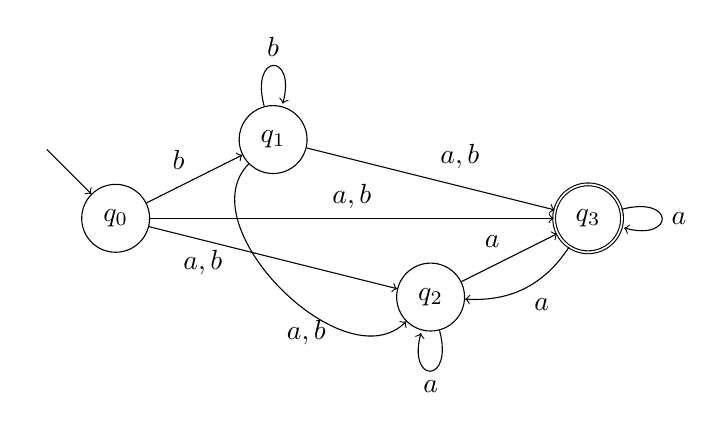
\begin{tikzpicture}[circle/.style={
                        shape=circle,
                        minimum size=0.5cm,
                        text=black, draw,
                        text width=0.5cm,
                        align=center}]
                        \node (vs) at (-1.0,1.0) {};
                        \node [circle] (q0) at (0,0) {$q_0$};
                        \node [circle] (q2) at (4,-1) {$q_2$};
                        \node [circle] (q1) at (2,1) {$q_1$};
                        \node [circle, double] (q3) at (6,0) {$q_3$};
                        \draw [->] (vs) edge (q0);
                        \draw [->] (q1) edge [loop above] node[auto] {$b$} (q1);
                        \draw [->] (q0) edge [bend left=0, pos=0.2] node[below] {$a,b$} (q2);
                        \draw [->] (q2) edge [bend left=0] node[auto] {$a$} (q3);
                        \draw [->] (q0) edge [bend left=0] node[auto] {$b$} (q1);
                        \draw [->] (q1) edge [bend left=0] node[auto] {$a,b$} (q3);
                        \draw [->] (q3) edge [bend left=30] node[auto] {$a$} (q2);
                        \draw [->] (q0) edge [bend left=0] node[auto] {$a,b$} (q3);
                        \draw [->] (q1) edge [bend right=90, pos=0.6] node[below] {$a,b$} (q2);
                        \draw [->] (q3) edge [loop right] node[auto] {$a$} (q3);
                        \draw [->] (q2) edge [loop below] node[auto] {$a$} (q2);
                        \qedhere
                \end{tikzpicture}
   \end{center}
\end{Bsp}



\begin{proof}[von \autoref{satz:2.EpsElim}: $\Eps$-Eliminierung]
        Zeige $L(\calN)=L(\B)$. Dabei verwenden wir die folgende Eigenschaft, die wir via Induktion über die Länge von $w$ in den Übungen zeigen werden.
        
        $\forall w\in\Sigma^+\; \forall q, q'\in Q:$
        $$(q,w,q')\in\reach_\B \Leftrightarrow \exists \underbrace{q_0, q_1,\ldots, q_n}_{\text{Lauf}}\in Q, \text{ sodass }  n=|w|, q_0=q \text{ und } q_n=q'$$
%         I.A. $(n=0,$ also $w=\Eps)$: Gilt trivialerweise da $(q,\Eps,q)\in\reach$ für alle $q$\\
%         I.S. ($n\rightsquigarrow n+1$): Seit $w=aw'$ beliebiges Wort der Länge $n+1$.
%         \begin{eqnarray*}
%                 (q,w,q')\in\reach\\
%                 & \Leftrightarrow & (q,w,q')\in\reach\\
%                 & \stackrel{\text{I.V.}}{\Leftrightarrow} & \exists\underbrace{q_1,q_2,\ldots, q_n}_{\text{Lauf}}\in Q, \text{ sodass }  n=|w'|, q_1\in \delta_\calP(p,a) \text{ und } q_n=q\\
%                 & \Leftrightarrow & \exists\underbrace{q_1,q_2,\ldots, q_n}_{\text{Lauf}}\in Q, \text{ sodass }  n=|w'|, \exists q_0\in p, \delta(q_0,a)=q_1 \text{ und } q_n=q\\
%                 & \Leftrightarrow & \exists\underbrace{q_0q_1,q_2,\ldots, q_n}_{\text{Lauf}}\in Q,\text{ sodass }  n+1=|w|, q_0\in p \text{ und } q_n=q
%         \end{eqnarray*}
        Mit Hilfe dieser Eigenschaft können wir nun leicht für $w \neq \varepsilon$ zeigen:
        \begin{eqnarray*}
         w\in L(\B) \hspace*{-1mm}
         &\stackrel{\text{\autoref{def:2.sprache}}}{\<=>} & \exists q_f\in F: (\qinit, w, q_f)\in\reach_\B\\
         &\<=> & \exists q_f\in F_\calN: \underbrace{q_0, q_1,\ldots, q_n}_{\text{Lauf}}\in Q, \text{ sodass }  n=|w|, q_0=\qinit \text{ und } q_n=q_f\\
         &\stackrel{\text{\autoref{def:2.EpsNeaSprache}}}{\<=>} & w \in L(\calN)
        \end{eqnarray*}
        Der Fall $w = \varepsilon$ folgt mit $\varepsilon \in L(\B) \Leftrightarrow \exists q \in F \cap \ecl_\B(\qinit) \Leftrightarrow \qinit \in F_\calN \Leftrightarrow \varepsilon \in L(\calN)$.
\end{proof}


\medskip

Mit Hilfe der $\Eps$-NEAs greifen wir nun die zu Beginn von Abschnitt~\ref{sec:2.EpsNea} aufgeworfene Fragestellung wieder auf und zeigen, dass für je zwei reguläre Sprachen auch die Konkatenation regulär ist.

Wir geben hierfür zunächst eine Konstruktion an.

\begin{Def}
Gegeben zwei $\Eps$-NEA $\B_i= (\Sigma, Q_i,\delta_i,\qinit_i,F_i)$, $i = 1,2$, definieren wir den \emph{$\Eps$-NEA für Konkatenation} $\B= (\Sigma, Q,\delta,\qinit,F)$ wie folgt.
                \begin{align*}
                Q &= Q_1 \overset.\cup Q_2\\
                \delta(q,a) &=
                                \begin{cases}
                                        \delta_1(q,a) & q\in Q_1\land (q\notin F_1 \lor a\neq \Eps)\\
                                        \delta_1(q,a)\cup\{\qinit_2\} & q\in F_1\land a=\Eps\\
                                        \delta_2(q,a) & q\in Q_2
                                \end{cases}\\
                \qinit & = \qinit_1\\
                F &= F_2 \qedhere
                \end{align*}
\end{Def}

\begin{Bsp} Der $\Eps$-NEA für Konkatenation für die beiden Automaten aus \autoref{bsp:2.naiveconcat} hat das folgende Zustandsdiagramm.
   \begin{center}
                \begin{tikzpicture}[circle/.style={
                        shape=circle,
                        minimum size=0.5cm,
                        text=black, draw,
                        text width=0.5cm,
                        align=center}]
                        \node (vs) at (-1.0,1.0) {};
                        \node [circle, fill=auto1] (v0) at (0,0) {$p_0$};
                        \node [circle, fill=auto1] (v1) at (2,0) {$p_1$};
                        \node [circle, fill=auto1] (v2) at (5,1) {$p_2$};
                        \node [circle, fill=auto1] (v3) at (5,-1) {$p_3$};
                        \draw [->] (vs) edge (v0);
                        \draw [->] (v0) edge [loop above] node[auto] {0} (v2);
                        \draw [->] (v0) edge [bend left=0] node[below] {1} (v1);
                        \draw [->] (v1) edge [bend left=15] node[auto] {0} (v2);
                        \draw [->] (v1) edge [bend left=0] node[below] {1} (v3);
                        \draw [->] (v2) edge [bend right=30] node[above] {0} (v0);
                        \draw [->] (v2) edge [bend left=15] node[auto] {1} (v1);
                        \draw [->] (v3) edge [bend left=0] node[right] {0} (v2);
                        \draw [->] (v3) edge [loop below] node[auto] {1} (v3);
                        \node [circle, fill=auto2] (s0) at (8,0) {$s_0$};
                        \node [circle, fill=auto2, accepting] (s1) at (11,0) {$s_1$};
                        \draw [->] (s0) edge [loop above] node[auto] {0} (s0);
                        \draw [->] (s1) edge [loop above] node[auto] {0} (s1);
                        \draw [->] (s0) edge [bend left=15] node[auto] {1} (s1);
                        \draw [->] (s1) edge [bend left=15] node[auto] {1} (s0);
                        
                        \draw [->] (v2) edge [bend left=0] node[auto] {$\Eps$} (s0);
                        \draw [->] (v3) edge [bend left=0] node[auto] {$\Eps$} (s0);
                        \qedhere
                \end{tikzpicture}
  \end{center}
\end{Bsp}


\begin{lemma}\label{satz:2.ClosedConcatenation}
Die vom $\Eps$-NEA für Konkatenation akzeptierte Sprache ist $L(\B_1)\cdot L(\B_2)$.
\end{lemma}
\begin{proof}
 Zeige via Induktion über die Länge von $w_1$, dass $\forall w_1,w_2\in\Sigma^*, \forall q_1\in Q_1, \linebreak[1] \forall q_1'\in F, \forall q_2'\in Q_2$ die folgende Eigenschaft gilt.
 \[
 (q_1,w_1,q_1')\in\reach_{\B_1} \text{ und } (\qinit,w_2,q_2')\in\reach_{\B_2} \quad\Leftrightarrow\quad (q_1,w,q_2')\in\reach_\B
 \qedhere
 \]
\end{proof}





\subsection{Abschlusseigenschaften}
\datenote{15.11.17}
% \begin{Def}[name={[Abgeschlossenheit von $\mathcal{L}$]}]
%         Eine Menge $\mathcal{L}\subseteq \mathcal{P}(\Sigma^*)$ von Sprachen heißt \emph{abgeschlossen} unter Operation \\
%         $f:\mathcal{P}(\Sigma^*)^n \-> \mathcal{P}(\Sigma^*)$ falls $\forall L_1,\dots, L_n\in \mathcal{L} : f(L_1,\dots, L_n)\in \mathcal{L}$.
% \end{Def}

\begin{Def}[name={[Abgeschlossenheit von $\mathcal{L}$]}]
        Eine Menge $X$ heißt \emph{abgeschlossen} unter Operation $f:X^n \-> X$, falls $\forall x_1,\dots, x_n\in X : f(x_1,\dots, x_n)\in X$.
\end{Def}
Zum Beispiel sind die natürlichen Zahlen abgeschlossen unter Addition, aber nicht abgeschlossen unter Subtraktion.

Im Folgenden schreiben wir $REG$ für die Menge aller regulären Sprachen.

\begin{lemma}\label{satz:2.ClosedComplement}
 Die Menge $REG$ der regulären Sprachen ist abgeschlossen unter Komplement.
\end{lemma}

\begin{proof}
Sei $L$ eine reguläre Sprache. 
Dann gibt es (per Definition) einen DEA $\A=(\Sigma, Q, \delta, \qinit, F)$ der L akzeptiert.
Wir konstruieren den DEA $\overline{\A}=(\Sigma, Q, \delta, \qinit, Q\backslash F)$ für $\overline{L}$, bei dem ein Zustand genau dann akzeptierend ist, wenn der Zustand in $\A$ nicht akzeptierend ist.
Man kann leicht zeigen, dass $L(\overline{\A})=\overline{L}$; somit ist auch $\overline{L}$ regulär.
\end{proof}

\begin{lemma}\label{satz:2.ClosedStar}
Die Menge $REG$ der regulären Sprache ist abgeschlossen unter dem Stern-Operator.
\end{lemma}

\begin{proof}
Sei $L$ eine reguläre Sprache. Dann gibt es einen $\Eps$-NEA $\B=(\Sigma, Q, \delta, \qinit, F)$, der $L$ akzeptiert. 
Wir konstruieren einen NEA $\B_*=(\Sigma, Q\overset.\cup\{\qinit_*\}, \delta_*, \qinit_*, F\overset.\cup\{\qinit_*\})$ für $L^*$, indem wir
\begin{itemize}
 \item einen neuen akzeptierenden Startzustand einführen,
 \item vom neuen Startzustand einen $\Eps$-Übergang zum alten Startzustand hinzufügen und
 \item von jedem akzeptierenden Zustand einen $\Eps$-Übergang zum alten Startzustand hinzufügen.
\end{itemize}
\[
                \delta_*(q,x) =
                        \begin{cases}
                                \delta(q,x) & q\notin F \text{ oder } x \neq \Eps\\
                                \{\qinit\} & q\in F \text{ und } x = \Eps \\
                                \{\qinit\} & q=\qinit_* \text{ und } x = \Eps
                        \end{cases}
\]
Man kann via Induktion über die Länge von Wörtern zeigen, dass $L(\B_*)=L^*$ gilt.
\end{proof}

Bemerkung: Die Menge der regulären Sprachen $REG$ ist unter den folgenden Operationen abgeschlossen.

\begin{center}
\begin{tabular}{cl@{\quad}l}
 $\cap$ & (Durchschnitt) & \autoref{satz:2.ClosedIntersection}\\
 $\cup$ & (Vereinigung) & Präsenzübungen erste Woche, Aufgabe~3\\
 $\overline{\phantom{X}}$ & (Komplement) & \autoref{satz:2.ClosedComplement}\\
 $\cdot$ & (Konkatenation) & \autoref{satz:2.ClosedConcatenation}\\
 $\phantom{\cdot}^*$ & (Kleene-Stern) & \autoref{satz:2.ClosedStar} 
\end{tabular}
\end{center}



% \begin{Satz}[name={[Abgeschlossenheit von $REG$]}]\label{satz:3.8}
%         Die Menge $REG$ der regulären Sprachen ist abgeschlossen unter $\cup$ (Vereinigung), $\cap$ (Durchschnitt), $\overline{\phantom{X}}$ (Komplement), Produkt (Konkatenation), Stern. Beispielsweise ist für $L_1, L_2$ reguläre Sprachen also auch $L_1 \cup L_2$, wie auch $L_1 \cap L_2$ etc. wieder eine reguläre Sprache.
% \end{Satz}
% \begin{proof}
% 	Sei $\A_i:=(Q_i,\Sigma,\delta_i,q_{0i},F_i)$, $\quad i=1,2$ \acs{NEA}s
% 	\begin{itemize}
% 	\item $\cup:$ Def $\A$ durch (vgl.\ Abb.~\ref{fig:reg-closure-union}):
% 		\begin{align*}
% 			Q &= Q_1\overset.\cup Q_2\overset.\cup\{q_0\}\\
% 			\delta(q,a) &=
%                 \begin{cases}
%                     \delta_1(q,a) & q\in Q_1\\
%                     \delta_2(q,a) & q\in Q_2\\
%                     \delta_1(q,a)\cup\delta_2(q,a) & q=q_0
%                         \end{cases}\\
%                         F &= F_1\overset.\cup F_2\overset.\cup (q_{01}\in F_1\lor q_{02}\in F_2) \rhd \{q_0\}
%                 \end{align*}
%                 Zeige $L(\A)=L(\A_1)\cup L(\A_2)$ (Aufgabe zum Eigenstudium: Betrachte die Läufe).
%                 \begin{figure}[tp]\centering
%                 \begin{tikzpicture}[>=stealth]
%                 \node (q0) at (0,0) {$q_0$};
%                 
%                 \node (q01) at (1.5,1.5) {$q_{01}$};
%                 \node (y) at (2.5,2) {$\bullet$};
%                 \node (x1) at (2.5,1) {$\bullet$};
%                 \node (qf1) at (4,1.5) {$q_{f_1}$};
%                 
%                 \node (q02) at (1.5,-1.5) {$q_{02}$};
%                 \node (x2) at (2.5,-1) {$\bullet$};
%                 \node (l) at (2.5,-2) {$\bullet$};
%                 \node (qf2) at (4,-1.5) {$q_{f_2}$};
%                 
%                 \path [->] (q0) edge [bend left=45] (y)
%                                 edge (x1)
%                                 edge (x2)
%                                 edge [bend right=45] (l)
%                           (q01) edge (y)
%                                 edge (x1)
%                           (q02) edge (x2)
%                                 edge (l)
% %                ;
% %                \path (q01) edge [bend left=80] (qf1)
% %                                    edge [bend right=80] (qf1)
%                 ;\draw (2.75,-1.5) ellipse (1.75 and 1.35);
%                 \node at (5,2) {$A_1$}
%                 ;
%                 \draw (2.75,1.5) ellipse (1.75 and 1.35);
%                 \node at (5,-1) {$A_2$};
%             \end{tikzpicture}
%             \caption{\acs{NEA} für Vereinigung}
%             \label{fig:reg-closure-union}
%         \end{figure}
%         \item $\cap:$ 
%         Annahme: Seien $\A_1$ und $\A_2$ zwei \acs*{DEA}s. Konstruiere nun  den \emph{Produktautomaten} $\A$, für den gilt (Aufgabe zum Eigenstudium!): $L(\A) = L(\A_1) \cap L(\A_2)$.
% 		\begin{align*}
% 			Q &= Q_1\x Q_2\\
% 			\delta((q_1,q_2),a) &= (\delta_1(q_1,a),\delta_2(q_2,a))\\
% 			q_0 &= (q_{01},q_{02})\\
% 			F &= F_1\x F_2\\
% 		\end{align*}
% 	\item Komplement: Ang. $\A_1$ ist \ac{DEA}, der $L$ erkennt. Ersetze $F_1$ durch $Q_1\setminus F_1$ und erhalte einen \acs*{DEA} $\A_1'$, der genau das Komplement von $L$ erkennt. 
% %
% %
%         \item Produkt: Seien $L_1$, $L_2$ regulär.\\
%                 Zeige $L_1\cdot L_2$ regulär.
%                 \begin{align*}
%                         Q &= Q_1 \overset.\cup Q_2\\
%                         \delta(q,a) &=
%                                 \begin{cases}
%                                         \delta_1(q,a) & q\in Q_1\setminus F_1\\
%                                         \delta_1(q,a)\cup\delta_2(q_{02},a) & q\in F_1\\
%                                         \delta_2(q,a) & q\in Q_2
%                                 \end{cases}\\
%                 q_0& = q_{01}\\
%                 F &= F_2\cup(q_{02}\in F_2) \rhd F_1
%                 \end{align*}
%                 Zeige $L(\A) = L(\A_1)\cdot L(A_2)$
%         \item Stern
%         \begin{align*}
%                 Q &= Q_1\overset.\cup \{q_0\}\\
%                 \delta(q,a) &=
%                         \begin{cases}
%                                 \delta_1(q,a) & q\in Q_1\setminus F_1\\
%                                 \delta_1(q,a)\cup\delta_1(q_{01},a) & q\in F_1\\
%                                 \delta_1(q_{01},a) & q=q_0
%                         \end{cases}\\
%                 F &= \{q_0\}\cup F_1\\
%                 \dots\ L(\A) &= L(\A_1)^*
%         \end{align*}
%         \end{itemize}
% \end{proof}
%

\renewcommand{\llbracket}{[\![}
\renewcommand{\rrbracket}{]\!]}

\subsection{Reguläre Ausdrücke}
\subsubsection{Motivation}
Problemstellung: Sie habe auf ihrem Rechner irgendwo eine Textdatei mit Notizen zu dieser Vorlesung, können sich aber grade nicht an den Pfad erinnern.
Sie wissen aber noch dass die Zeichenkette \texttt{info3} oder \texttt{infoIII} enthalten ist. 
Möglicherweise war das \texttt{i} am Anfang aber auch groß geschrieben.
Da sie ein paar Dateien mit dieser Zeichenkette haben soll der Rechner jeweils Dateinamen und die entsprechenden Zeilen ausgeben.

Auf Systemen auf denen die GNU Tools installiert sind kann dieses Problem mit dem Befehl \texttt{find ....} gelöst werden.

Konzeptuell soll ihr Rechner hier instanzen des Wortproblem lösen.
Ihre Sprache sind alle Zeichenketten die \texttt{info3} in den oben beschriebenen Variationen enthalten.
Ihre Wörter sind die Zeilen aller Dateien auf dem Rechner.

Eine Umsetung: Gib Rechner den folgenden NEA ...


...

\begin{Def}[name={[RE($\Sigma$)]}]
        Die Menge $RE(\Sigma)$ der \emph{regulären Ausdrücke über $\Sigma$} ist induktiv definiert durch:
        \begin{itemize}
        \item $\0\in RE(\Sigma)$
        \item $\1\in RE(\Sigma)$
        \item $a\in RE(\Sigma)$ für alle $a\in\Sigma$
        \item falls $r,s\in RE(\Sigma)$
                \begin{itemize}[label=\textbullet]
                \item $(r+s)\in RE(\Sigma)$
                \item $(r\cdot s)\in RE(\Sigma)$
                \item $(r)^*\in RE(\Sigma)$
                \end{itemize}
        \end{itemize}
\end{Def}
Konventionen: Wir möchten nicht immer alle Klammern schreiben müssen. 
Wir führen deshalb die folgenden Präzedenzregeln ein: ``$\strut^*$'' bindet stärker als ``$\cdot$'' und ``$\cdot$'' bindet stärker als ``$+$''.
Nach Definition der Semantik werden wir außerdem sehen, dass ``$\cdot$'' und ``$+$'' assoziativ sind. 
Unsere Konvention ist: 
Sofern mit Hilfe dieser Regeln der reguläre Ausdruck zweifelsfrei rekonstruiert werden kann dürfen wir Klammern und ``$\cdot$'' weglassen.
Wir schreiben z.B. $110 + 0$ statt $((1\cdot (1\cdot 0)) + 0)$

\begin{Bsp}~

$\0\1\0\1$ ist ein regulärer Ausdruck

$a^4b^7$ ist kein regulärer Ausdruck
\end{Bsp}


\begin{Def}[name={[Semantik eines regulären Ausdrucks]}]
        Die Semantik eines regulären Ausdrucks $\llbracket\cdot \rrbracket : RE(\Sigma) \-> \mathcal{P}(\Sigma^*)$ ist induktiv definiert durch
        \begin{align*}
                \llbracket \0 \rrbracket &= \varnothing\\
                \llbracket \1 \rrbracket &= \{\Eps\}\\
                \llbracket a \rrbracket &= \{a\} \quad a\in\Sigma\\
                \llbracket r+s \rrbracket &= \llbracket r\rrbracket \cup \llbracket s\rrbracket\\
                \llbracket r\cdot s \rrbracket &= \llbracket r\rrbracket \cdot \llbracket s\rrbracket\\
                \llbracket r^* \rrbracket &= \llbracket r\rrbracket^* \qedhere
        \end{align*}
\end{Def}
%
    \begin{Bsp*} Mustererkennung
        \begin{itemize}
        \item Akzeptiere alle Wörter, die $abac$ enthalten: 
        \begin{align*} & \Sigma^* abac \Sigma^* \\
                       \Leftrightarrow & (a_1 + a_2 + ...)^* abac (a_1 + a_2 + ...)^* \forall a_i \in \Sigma
          \end{align*}
        \item Sei $\Sigma=\{0,1\}$. Die Sprache aller Wörter, deren $n$-letztes Symbol = 1, ist nicht regulär, denn:
        \begin{gather*}
        (0+1)^*1\underbrace{(0+1)\dots(0+1)}_{n-1}\\
        \xcancel{0^n1^n}\notin RE(\Sigma)
        \end{gather*}
        \item Ein regulärer Ausdrück für alle Wörter $\omega \in (0, 1)^*$, s.d. $\omega \mod 3=0$:
        \[ (0+1(01^*0)^*1)^* \]
        
    \captionsetup{type=figure}
    \begin{tikzpicture}[>=stealth, shorten >=1pt, on grid, node distance=2cm, initial text=]
        \node[state, initial, accepting] (q0) {$q_0$};
        \node[state] (q1) [right=of q0] {$q_1$};
        \node[state] (q2) [right=of q1] {$q_2$};
        \path [->]
            (q0) edge[loop below] node[auto] {0} ()
                 edge[bend left]  node[auto] {1} (q1)
            (q1) edge[bend left]  node[auto] {0} (q2)
                 edge[bend left]  node[auto] {1} (q0)
            (q2) edge[loop right] node[auto] {1} ()
                 edge[bend left]  node[auto] {0} (q1)
        ;
        
        \draw [->,decorate,decoration=snake] ($(q1.south) - (0,.5cm)$) -- ++(0,-1cm);
        
        \node [state, initial, accepting] (q0) [below=3cm of q0] {$q_0$};
        \node [state] (q1) [right=of q0] {$q_1$};
        \path [->]
            (q0) edge[loop below] node[auto] {0} ()
                 edge[bend left]  node[auto] {1} (q1)
            (q1) edge[loop right] node[auto] {$01^*0$} ()
                 edge[bend left]  node[auto] {1} (q0)
        ;
        
        \node [state, initial, accepting] (q0) [below=2.5cm of q0] {$q_0$};
        \path [->]
            (q0) edge[loop below] node[auto] {0} ()
                 edge[loop right] node[auto] {$1(01^*0)^*1$} ()
        ;
    \end{tikzpicture}
    \captionof{figure}{Informell vom Automaten zum regulären Ausdruck für mod 3}
  \qedhere
\end{itemize}
    \end{Bsp*}
\begin{Satz}[Kleene]
$L$ ist regulär \<=> $L$ ist Sprache eines regulären Ausdrucks.
\end{Satz}


\begin{proof}[Kleene, $\<=$]
Betrachte zu einem regulärem Ausdruck $r\in RE(\Sigma)$ die durch diesen erzeugte Sprache $L=\llbracket r \rrbracket$. Zeige per Induktion über $r$, dass $ \forall r\in RE(\Sigma) $ gilt: $ \llbracket r \rrbracket$ ist regulär.
    	\begin{description}[font=\normalfont]
      \item[I.A.:] \hfill
        \vspace{-\baselineskip}
        \begin{itemize}
        \item $r = \0$, $\llbracket r \rrbracket = \emptyset$ ist regulär
        \item $r = \1$, $\llbracket r \rrbracket = \{ \Eps \}$ ist regulär
        \item $r = a$, $\llbracket r \rrbracket = \{ a \}$ ist regulär \\
          (\tikz[>=stealth, shorten >=1pt, initial text=,
    					on grid, baseline=-.6ex,
    					every state/.style={minimum size=0pt,inner sep=0pt}
    				]{
    				\node [state,initial] (a) {}; \node [state,accepting] (b) [right=of a] {};
    				\path [->] (a) edge node [auto] {$a$} (b);
    			}
    			 \quad\acs{NEA}) 
        \end{itemize}
        \item[I.V.:] Für $i \in \{1, 2\}$ gilt: $\llbracket r_i \rrbracket$ ist regulär.
    		\item[I.S.:] \hfill
          \vspace{-\baselineskip}
          \begin{itemize}
          \item $r = r_1 + r_2$, $\llbracket r \rrbracket = \llbracket r_1 \rrbracket \cup \llbracket r_2 \rrbracket$ ist regulär nach \autoref{satz:3.8}
          \item $r = r_1 \cdot r_2$, $\llbracket r \rrbracket = \llbracket r_1 \rrbracket \cdot \llbracket r_2 \rrbracket$ ist regulär nach \autoref{satz:3.8}
          \item $r = r_1^*$, $\llbracket r \rrbracket = \llbracket r_1 \rrbracket^*$ ist regulär nach \autoref{satz:3.8}
          \end{itemize}
		\end{description}
\end{proof}

Zum Beweis (bzw.\ zur Konstruktion) der Richtung "`\=>"' benötigen wir eine Rechenregel zum Lösen von Gleichungen zwischen regulären Sprachen und Ausdrücken:
\begin{lemma}[Ardens Lemma]\label{lem:arden}\ \\
        Sei die lineare Gleichung $X=A\cdot X+B$ über $A, B, X\subseteq \Sigma^*$ gegeben. Dann ist $X=A^*B$ eine Lösung. Falls $\Eps \notin A$ ist diese Lösung ausserdem eindeutig.
\end{lemma}

\begin{proof}
Sei $ X= AX+B$ mit $\Eps\notin A$. Zeige, dass $A^*B \subseteq X$:
        \begin{alignat*}{3}
                && A^*B &= AA^*B + B = (\1+AA^*)B = B+A(A^*B) \quad\checkmark\\
                \shortintertext{Angenommen $A^*B \subsetneq X$, d.h.\ $\exists w\in X$ mit $w\notin A^*B$, davon sei $w$ das kürzeste.}
                \exists n\geq 1: && X &= \underbrace{A^nX}_{\ni w} + \underbrace{A^{n-1}B+\dots +AB+B}_{\not\ni w}\\
                \curvearrowright && w &= u_1\dots u_n w'\text{ mit } u_1,\dots,u_n\in A\text{ und } w'\in X\\
                \curvearrowright && |w'| &< |w|\\
                \text{Falls}&& w'&\in A^*B \curvearrowright w\in A^nA^*B\subseteq A^*B \quad \lightning\\
                \text{Also} && w'&\notin A^*B \quad\lightning\text{ gegen Minimalität von }w\\
                \curvearrowright && X&\subseteq A^*B\\
                \-> && X &= A^*B
                \qedherefixalignat
        \end{alignat*}
\end{proof}

\begin{Korollar}
  Ardens Lemma lässt sich auch für reguläre Ausdrücke formulieren: Seien $r_X,r_A,r_B$ reguläre Ausdrücke mit $\Eps \not \in \llbracket r_A \rrbracket$ für die die folgende Gleichung gilt:
  \begin{displaymath}
    \llbracket r_x \rrbracket = \llbracket r_A \cdot r_x + r_B \rrbracket
  \end{displaymath}
  Dann ist 
  \begin{displaymath}
    r_x := r_A^*r_B
  \end{displaymath}
  eine eindeutige Lösung für $r_x$, die die Gleichung erfüllt.
\end{Korollar}

% \datenote{11.11.16}

\begin{proof}[Kleene, \=>]
  Sei $L=L(\A)$ für einen \ac{DEA} $\A=({Q},\Sigma,\delta,q_0,F)$ mit $Q = \{q_0,q_1,\dots,q_n\}$.
        Definiere $L_i=\{ w \mid \tilde\delta(q_i,w)\in F \}$ als die Sprache der Wörter, die von Zustand $q_i$ aus in einen akzeptierenden Zustand führen.
  Insbesondere gilt $L_0 = L$.

  Wir leiten nun ein lineares Gleichungssystem zwischen den Sprachen $L_i$ her.
  Zunächst teilen wir $Li$ in den Teil der (potentiell) das leere Wort enthält und den, der die nicht-leeren Wörter enthält.
  \begin{align*}
    L_i & =  \{ w \mid \tilde\delta(q_i,w)\in F \} \\
        & =  \{ \Eps \mid \tilde\delta(q_i, \Eps) \in F \} \cup \{a w' \mid a \in \Sigma, w' \in \Sigma^*, \tilde\delta(\delta(q_i, a), w') \in F\} \\
        & =  \{ \Eps \mid q_i \in F \} \cup \{a w' \mid a \in \Sigma, w' \in \Sigma^*, \tilde\delta(\delta(q_i, a), w') \in F\}
    \end{align*}
    Die nicht-leeren Wörter hängen von den Sprachen der Folgezustände ab:
    \begin{align*}
      \{a w' \mid a \in \Sigma, w' \in \Sigma^*, \tilde\delta(\delta(q_i, a), w') \in F\} & =
         \bigcup_{a \in \Sigma} \{a\} \{w' \mid a \in \Sigma, w' \in \Sigma^*, \tilde\delta(\delta(q_i, a), w') \in F\}
      \\
      & = \bigcup_{a \in \Sigma} \{a\} (L_j \text{ wobei  $q_j = \delta(q_i, a)$}) 
    \end{align*}
    Anstatt die Vereinigung über die Transitionen $a$ und Folgezustandssprachen $L_j$ zu bilden, lassen sich die nicht-leeren Wörter von $L_i$ auch als Vereinigung über aller Zustände mit entsprechend gewählten \emph{Koeffizienten} formulieren; die Zustände die keine Folgezustände sind, habe den Koeffizienten $\emptyset$.
    \begin{align*}
      \bigcup_{a \in \Sigma} \{a\} (L_j \text{ wobei  $q_j = \delta(q_i, a)$}) & = \bigcup_{j = 0}^{n} \underbrace{\{a \mid a \in \Sigma, \delta(q_i, a) = q_j\}}_{A_{ij} \not \ni \Eps} L_j
    \end{align*}
    Man beachte das die Koeffizienten $A_{ij}$ nie das leere Wort enthalten.
    Nach diesen Überlegungen ergibt sich also für die Sprachen $L_i$ das lineare Gleichungssystem
    \begin{displaymath}
      L_i = \{ \Eps \mid q_i \in F \} \cup \bigcup_{j = 0}^{n} \underbrace{\{a \mid a \in \Sigma, \delta(q_i, a) = q_j\}}_{A_{ij} \not \ni \Eps} L_j
    \end{displaymath}
    Diese Gleichungen lassen sich analog als Gleichungen von regulären Ausdrücken $r_i$ formulieren:
    \begin{align*}
      r_i &= N(q_i) + \sum_{j = 0}^n R_{ij} r_j
    \end{align*}
    wobei $\llbracket r_i \rrbracket = L_i$ und $R_{ij } = \sum \{a \mid a \in \Sigma, \delta(q_i, a) = q_j\}$ mit $\Eps \not \in \llbracket R_{ij} \rrbracket$ und
    \begin{displaymath}
      N(q_i) =
      \begin{cases}
        \1 & q_i\in F\\
        \0 & q_i\notin F
      \end{cases}
    \end{displaymath}
    Dieses Gleichungssystem lässt sich, wie lineare Gleichungssysteme in der Arithmetik, mit dem \emph{Substituitionsverfahren} lösen ("`auflösen nach einer Variablen und einsetzen"').
    Dazu werden Ardens Lemma und weitere Rechenregeln für Sprachen, wie Distributivität, verwendet.
    Wir beginnen mit Gleichung $r_n$:
    \begin{align*}
      r_n &= N(q_n) + \sum_{j = 0}^n R_{nj} r_j \\
          &= \underbrace{N(q_n) + \left (\sum_{j = 0}^{n-1} R_{nj} r_j \right)}_{r_B} + \underbrace{R_{nn}}_{r_A} r_n
    \end{align*}
    Wie oben angedeutet ist nach dem Herausziehen des $n$ten Summenglieds Ardens Lemma anwendbar (merke, $\Eps \not \in \llbracket R_{nn} \rrbracket$), und wir setzen:
    \begin{displaymath}
      r_n := R_{nn}^*\left(N(q_n) + \sum_{j = 0}^{n-1} R_{nj} r_j  \right)
    \end{displaymath}
    Dieses Ergebnis in $r_0,\ldots,r_{n-1}$ eingesetzt ergibt:
    \begin{align*}
      r_i &= N(q_i) + \left (\sum_{j = 0}^{n-1} R_{nj} r_j \right) + R_{in}R_{nn}^*\left(N(q_n) + \sum_{j = 0}^{n-1} R_{nj} r_j  \right) \\
      \intertext{(Ausmultiplizieren von $R_{in}R_{nn}^*$)}
          &= N(q_i) + \left (\sum_{j = 0}^{n-1} R_{nj} r_j \right) + R_{in}R_{nn}^*N(q_n) + \sum_{j = 0}^{n-1} R_{in}R_{nn}^*R_{nj} r_j  \\
      \intertext{(Zusammenlegen der Summen und Ausklammern von $r_j$)}
          &= N(q_i) + R_{in}R_{nn}^*N(q_n) + \sum_{j = 0}^{n-1} (R_{nj} + R_{in}R_{nn}^*R_{nj}) r_j  \\
    \end{align*}
  Nach diesen Umformungen ergeben sich $\Eps$-freie Koeffizienten $R_{nj} + R_{in}R_{nn}^*R_{nj}$ für $r_j$ und wir mit dem Auflösen von $n-1$ analog zu $n$ fortfahren.
  Am Ende erhalten wir einen regulären Ausdruck als Lösung für $r_0$.
  Per Konstruktion haben wir immer noch $\llbracket r_0 \rrbracket = L_0 = L$.
  \end{proof}
    

\begin{Bsp*} Ein Beispiel für die Konvertierung eines \ac{DEA} in einen reg. Ausdruck.
	\begin{figure}[H]\centering
		\begin{tikzpicture}[>=stealth, shorten >=1pt, on grid, node distance=2cm, initial text=]
			\node[state, initial, accepting] (q0) {$q_0$};
			\node[state] (q1) [right=of q0] {$q_1$};
			\node[state] (q2) [right=of q1] {$q_2$};
			\path [->]
			    (q0) edge[loop above] node[auto] {0} ()
			         edge[bend left]  node[auto] {1} (q1)
			    (q1) edge[bend left]  node[auto] {0} (q2)
			         edge[bend left]  node[auto] {1} (q0)
			    (q2) edge[loop right] node[auto] {1} ()
			         edge[bend left]  node[auto] {0} (q1)
			;
		\end{tikzpicture}
		\caption{\ac{DEA} "`modulo 3"'}
	\end{figure}
	lineares Gleichungssystem mit 3 Unbekannten.
	\begin{align*}
		L_0 &= \1 + 0\cdot L_0 + 1\cdot L_1\\
		L_1 &= 1\cdot L_0 + 0\cdot L_2\\
		L_2 &= \underbrace{0\cdot L_1}_B + \underbrace{1}_A\cdot L_2\\
		\shortintertext{\nameref{lem:arden} auf $q_2$:}
		L_2 &= 1^*\cdot 0\cdot L_1\\
		\shortintertext{Einsetzen in $q_1$}
		L_1 &= \underbrace{1\cdot L_0}_B+\underbrace{0\cdot 1^*\cdot 0}_A\cdot L_1\\
		\shortintertext{\nameref{lem:arden} auf $q_1$:}
		L_1 &= (01^*0)^*\cdot 1\cdot L_0\\
		\shortintertext{Einsetzen:}
		L_0 &= \1 + 0\cdot L_0+1\cdot (01^*0)^*\cdot 1\cdot L_0\\
		&= \1+(0+1\cdot (01^*0)^*\cdot 1)\cdot L_0\\
		\shortintertext{\nameref{lem:arden} auf $q_0$:}
		L_0 &= (0+1\cdot (01^*0)^*\cdot 1)^*
		\qedhere
	\end{align*}
\end{Bsp*}
%
\hide{
\draftnote{11.11.16}
\subsection{Entscheidungsprobleme}
Ein Problem ist \emph{entscheidbar} wenn es sich durch eine binäre Antwort (ja/nein) lösen lässt und es einen Algorithmus gibt, der für alle Instanzen des Problem die korrekte Antwort liefert.
\begin{Satz}[name={[Wortproblem]}]\label{satz:wortproblem}
        Das Wortproblem ist für reguläre Sprachen entscheidbar.
        
        D.h. Falls $L$ reg. Sprache und $w\in\Sigma^*$, dann ex. Algorithmus, der entscheidet, ob $w\in L$.
\end{Satz}
\begin{proof}
	$L$ sei durch \ac{DEA} gegeben.\\
	Berechnung von $\tilde\delta(q_0,w)$ entspricht Durchlauf durch Graph des \ac{DEA} + Test ob erreichter Zustand $\in F$ in Zeit $O(n)\ ,\ n=|w|$.
\end{proof}

\begin{Satz}[name={[Leerheitsproblem]}]\label{satz:leerheitsproblem}
        Das \emph{Leerheitsproblem} ist für reg. Sprachen entscheidbar.
        Falls $L$ reg. Sprache, dann existiert ein Algorithmus, der entscheidet, ob $L=\varnothing$.
\end{Satz}
\begin{proof}
	Sei $\A$ \ac{DEA} für $L$.\\
	Setze Tiefensuche auf den Graphen von $\A$ an. Start bei $q_0$.\\
	Falls die Suche einem akzeptierenden Zustand findet: Nein.\\
	Ansonsten: Ja: $L=\varnothing$\\
	Zeit: $O(|\Sigma||Q|)$
\end{proof}

\begin{Satz}[name={[Endlichkeitsproblem]}]\label{satz:endlichkeitsproblem}
        Das Endlichkeitsproblem für reg. Sprachen ist entscheidbar.
\end{Satz}
\begin{proof}
	Falls $L$ durch $r\in RE(\Sigma)$ gegeben.\\
	$r$ enthält keinen $^* \=> \llbracket r \rrbracket$ endlich.\\
	Zeit: $O(|r|)$
	
	[Reicht nicht, liefert nur eine Richtung]
	
	Falls $L$ durch \ac{DEA} $\A$ gegeben.
	
	\begin{tikzpicture}[>=stealth]
		\node (q0) {$q_0$};
		\node (q1)  [right=.75cm of q0]{$\cdot$};
		\node (q2) [right=.48cm of q1] {$\times$};
		\node (q3) [below=.4cm of q2, xshift=.4cm, inner sep=0pt] {$\times$};
		\draw[->] (q0) edge (q1)
			(q2) ++(-.1cm,-.3cm) -- (q3);
		\draw[->] (q1.south) arc (-155:155:.5cm);
	\end{tikzpicture}
	
	\paragraph*{Oder:} mit \nameref{lem:pumping}.\\
	Sei $L$ regulär und $n$ die Konstante aus dem \ac{PL}.\\
	$L$ unendlich \<=> $\exists w\in L : n\leq |w| <2n$
	\begin{description}[font=\normalfont,labelwidth=\widthof{"'\<="':},leftmargin=!]
	\item["'\<="':] $w$ erfüllt Voraussetzung des \ac{PL}, also $w=uvx$ mit $|uv|\leq n$ und $|v|\geq 1$.\\
		Nach \ac{PL}: $\forall i\in\N: uv^ix\in L$, also $L$ unendlich.
	\item["'\=>"'] \emph{Angenommen} $L$ unendlich, aber $\forall w\in L : |w|<n$ oder $|w|\geq 2 n$\\
	Sei $w\in L$ minimal gewählt, sodass $|w|\geq 2n$.
	
	$w$ erfüllt Voraussetzung vom \ac{PL}, also $w=xyz$ mit $|xy|\leq n$ und $|y|\geq 1$\\
	also $\forall i\in\N: xy^iz\in L$ insbes. $i=0: xz\in L$ mit $|xz|<|w|$.
	
	Zwei Möglichkeiten:
	\begin{enumerate}[label=(\alph*)]
	\item $|xz|\geq 2n\ \lightning$ Minimalität von $w$
	\item $|xz|<2n$
		\begin{align*}
			|xz|+|y| &= |w|\geq 2n\text{ mit } 1\leq|y|\leq n\\ %TODO warum gilt 1\leq|y|\leq n ??
			\Rightarrow |xz| &= |w|-|y|\geq 2n-n=n \\
			\Rightarrow |xz| & \geq n \wedge |xz| < 2n \quad\lightning\text{zur Annahme}
		\end{align*}
		Also $\exists w\in L$ mit $n\leq|w|<2n$ \qedhere
	\end{enumerate}
	\end{description}
\end{proof}

\begin{Satz}[name={[Schnittproblem]}]\label{satz:schnittproblem}
        Das \emph{Schnittproblem} ist für REG entscheidbar.\\
        D.h. $L_1,L_2$ reguläre Sprachen. Ist $L_1\cap L_2 = \varnothing$?
\end{Satz}
\begin{proof}
        Nach Satz~\ref{satz:schnittproblem} ist $L_1\cap L_2$ regulär. $L_1\cap L_2=\varnothing$ entscheidbar nach \autoref{satz:leerheitsproblem}.
\end{proof}

\begin{Satz}[name={[Äquivalenzproblem]}]\label{satz:äquivalenzproblem}
	Das \emph{Äquivalenzproblem} ist für REG entscheidbar.\\
	D.h. gegeben \ac{DEA}s für $L_1$ und $L_2$, $\A_1$ und $\A_2$
	\[ L_1 = L(\A_1) = L(\A_2) = L_2\ ? \qquad \framebox{Inklusionsproblem}\]
\end{Satz}
\vspace{-2em}
\begin{proof}
        \begin{alignat*}{3}
                L_1\cap \overline{L}_2 &= \varnothing &\quad&\<=>\quad & L_1 &\subseteq L_2\\
                (L_1\cap\overline{L}_2)\cup(L_2\cap \overline{L}_1) &= \varnothing &&\<=> & L_1 &= L_2
                \qedherefixalignat
        \end{alignat*}
\end{proof}

\begin{Satz}[name={[Inklusionsproblem]}] Äquivalenzproblem \<=> Inklusionsproblem (für REG)
\end{Satz}
\begin{proof}
\begin{itemize}
\item  $=$ entspricht $\subseteq\land\supseteq$
\item $L_1 \subseteq L_2$ genau dann, wenn $L_1 \cup L_2 = L_2$; REG ist abgeschlossen unter Vereinigung
\end{itemize}
\end{proof}


Anwendungsbeispiel für reguläre Sprachen.

$N$ -- liest vom Netz\\
$R$ -- liest lokalen Speicher (ggf. vertrauliche Info)\\
$W$ -- postet auf FB

Programm:

\begin{tabular}{M{l}@{}M{l}@{}M{l}}
        p = N | R | W &| \text{ if }&* \text{ then } p_1\\
        &&\phantom{*}\text{ else }p_2\\
        &|\text{ while }&*\text{ do }p\\
        \mathrlap{
                \begin{rcases}
                        \text{while }*\text{ do }N;\\
                        R;\\
                        \text{if }*\text{ then }N\text{ else }W
                \end{rcases} N^*R\cdot (N+W)
        }
\end{tabular}

Sicherheitspolitik: nach Lesen von lokalem Speicher kein Posten auf FB  $\overline{\Sigma^*R\Sigma^*W\Sigma^*}$

Programm erfüllt Sicherheitspolitik nicht, denn
\[
        \underset{\underset{\displaystyle N^*RW}{\rotatebox[origin=c]{-90}{$\supseteq$}}}{N^*\cdot R(N+W)} \not\subseteq \overline{\Sigma^*R\Sigma^*W\Sigma^*}
\]
}

%%% Local Variables:
%%% mode: latex
%%% TeX-master: "Info_3_Skript_WS2016-17"
%%% End:
